%==================================================================================================
%   THESIS TEMPLATE
%   -------------------------
%   This template is based upon the offcial IMM PhD Thesis template, it is enhanced with a number 
%   of new features and a number of errors have fixed. This template is intended to be complied to 
%   PDF using PDFLATEX and is tested using the MiKTeX 2.9 LaTeX distribution. 
%   It is based on the official DTU-IMM Thesis template by Finn Kuno Christensen in 2009. 
%==================================================================================================
%
%==================================================================================================
% DOCUMENT SETUP
%==================================================================================================
\documentclass[10pt,twoside]{book}                  %Official DTU-IMM Thesis document setup
%
%Set to 'print' for printed version, use 'net' for online version
\def\thesisversion{print} 			
%
%==================================================================================================
% PACKAGES
%==================================================================================================
\usepackage{ImmThesis}                              %Import Thesis base style 

%==================================================================================================
% THESIS PROPERTIES (Modifiy these fields with your details)
%==================================================================================================
\def\thesisauthor{Niklas Christoffer Petersen}            %Author 
\def\thesistitle{A Logical Approach to Sentiment Analysis}      %Title
\def\thesishandin{September 30}                       %Submission date (Day-Month}
\def\thesisyear{2012}                             %Submission year 
\def\thesisnumber{126}                            %DTU-IMM Serial number (do not include year)
\def\thesisISSN{0000-0000}                          %ISSN number
\def\thesiskeywords{Keywords are, comma separated}  %PDF keywords 
\derivethesisprops                                  %Derive dependent properties
%
%==================================================================================================
% SECTION NUMBERING SETUP
%==================================================================================================
\setcounter{tocdepth}{2}                            %2 adds sections up to subsections
\setcounter{secnumdepth}{3}                         %Subsubsections get a number when this is 3
%
%==================================================================================================
% THESIS STRUCTURE  (Modifiy to include more chapters etc)
%==================================================================================================

\usepackage{named}

\usepackage{framed}
\usepackage{enumitem}
\usepackage[textwidth=2cm]{todonotes}
\usepackage{tikz}
\usetikzlibrary{backgrounds}
\usepackage{xifthen}

\usepackage{siunitx}

% Figures, graphs, etc.
%\usepackage[landscape]{geometry}
\usepackage{rotating}
\usepackage{longtable}
\usepackage{color}
\usepackage{pgfplots}

% Code
\usepackage{listingsutf8}
\usepackage{clrscode3e}


% Pdf
\ifx\thesisversion\printversion
  \usepackage{lscape}
\else
  \usepackage{pdflscape}
\fi

\lstdefinelanguage{GHC}{
  morekeywords={module,import,qualified,as,hiding,let,return,data,type,case,of,infix,deriving,class,where,do,instance},
  sensitive=true,
  morecomment=[l]{--},
  morestring=[b]",
}

\lstset{language=GHC,basicstyle=\ttfamily\scriptsize, breaklines=true,
  keywordstyle=\bf\color{blue},tabsize=2,columns=fixed,commentstyle=\color{gray}}
\lstdefinelanguage{text}{}

\newenvironment{numquote}
{%	
	\par
	\refstepcounter{equation}
	\hspace{.5cm}
    \begin{minipage}[c]{10cm}        	
    	\em
}
{%
	\end{minipage}
	\hfill 	
	(\arabic{chapter}.\arabic{equation})\\[0mm]
}

\newenvironment{numquote1}
{%  
  \par
  \refstepcounter{equation}
  \hspace{.5cm}
    \begin{minipage}[b]{10cm}
      \em
}
{%
    \end{minipage}
  \hfill  
  (\arabic{chapter}.\arabic{equation})%\\[0mm]
}

\newenvironment{cframed}[1]
{%
	\begin{center}	
	\begin{minipage}[b]{#1}
		\begin{framed}		
}
{%
			\vspace{-1em}
		\end{framed}
	\end{minipage}	
	\end{center}
	\vspace{-1em}
}


\newcommand{\con}{\wedge}
\newcommand{\dis}{\vee}
\newcommand{\pr}{\rightarrow}
\newcommand{\assign}{\leftarrow}

%\newcommand{\bsl}{\text{\textbackslash}}
\newcommand{\bsl}{\backslash}

\newcommand{\cat}[1]{{\mathit{#1}}}
\newcommand{\catvar}[1]{\makebox[1em]{$#1$}}
\newcommand{\fvar}[1]{\makebox[8pt]{$#1$}}
\newcommand{\token}[1]{\mathbf{#1}}
\newcommand{\pos}[1]{\scriptstyle{\mathbf{#1}}}

\newcommand{\inference}[3][]{
  \ifthenelse{\equal{#1}{T}}
  {
  	\begin{array}{c} 
  		\vspace{-4pt}
  		#2 \\
  		\vspace{-4pt}
  		\triangledown \\  		
  		#3
  	\end{array}
  }
  {
  	\dfrac{\! \begin{array}{c} #2 \end{array} \!}{\! \begin{array}{c} #3 \end{array} \!}
  	\ifthenelse{\isempty{#1}}
  	{ \: } % if #1 is empty
  	{\hspace{-6pt}\begin{array}{l}\scriptscriptstyle{\mathbf{#1}} \\ \vspace{-9.6pt} \end{array}} % if #1 is not empty
  }
}

\begin{document}
%------------------------                                    
%Pre-frontmatter material
%------------------------
\prefrontmatter
%--------------------
%Frontmatter material
%--------------------
\frontmatter
\pagenumbering{roman}                               %Set frontmatter numbering style
%!TEX root = Thesis.tex

\chapter{Summary (English)}

	The goal of the thesis is to ...								             %English summary of Thesis
\markboth{}{}                                       %Set headings (left)(right)
%!TEX root = Thesis.tex

\chapter{Summary (Danish)}
\begin{otherlanguage}{danish}

Målet for denne afhandling er at ...




\end{otherlanguage}								             %Danish summary of Thesis
\markboth{}{}                                       %Set headings (left)(right)
%!TEX root = Thesis.tex

\chapter{Preface}

This thesis was prepared at the department of Informatics and Mathematical Modelling at the Technical University of Denmark in partial fulfilment of the
requirements for acquiring an MSc in Computer Science and Engineering. 

The thesis deals with ... 

The thesis consists of ...

Furthermore three project-specific learning objectives for the project concerned should be presented. The following is simply suggestions for those:
\begin{itemize}
	\item Understand and extend modern techniques for processing of natural language texts using formal logical systems.

	\item Demonstrate methods for formal reasoning with respect to natural language understanding.
	
	\item Present a \emph{proof of concept} system, that is a fully functional implementation of essential theoretical presented methods.
\end{itemize}

%==================================================================================================
% SIGNATURE AREA
%==================================================================================================
\vspace{20mm}
\begin{center}
	\hspace{20mm} Kgs. Lyngby, \thesishandin, \thesisyear 
	\vspace{5mm}
	\newline
 

%	
\includegraphics[scale=0.5]{Figures/Signature}
\end{center}
\begin{flushright}
	\vspace{6em}
	\thesisauthor
\end{flushright}
% % % EOF % % %								             %Preface
\markboth{}{}                                       %Set headings (left)(right)
%!TEX root = Thesis.tex

\chapter{Acknowledgements}

I would like to thank Jørgen Villadsen for his help and guidance during the entire project, and for his lectures in the course Formal Logical Systems (02156) which sparked my interest in the area of formal logic and later lead to my deep interest in computational linguistics. Also the courses Program Analysis (02242) and Functional Programming (02157) have contributed with knowledge crucial to the completion of my thesis. Finally I attended the 24th European Summer School in Logic, Language and Information (ESSLII) in Opole, Poland during the project, which also provided highly advanced knowledge that has been applied in this thesis.

I would also like to give thanks to Henriette Jensen and Johannes Svante Spurkeland for providing test data by individually labeling review texts. Further thanks to Mchael Lunøe and Johannes Svante Spurkeland for constructive feedback during this thesis.					             %Acknowledgements
\markboth{}{}                                       %Set headings (left)(right)
%------------------
% Table of contents
%------------------
\newpage\mbox{}\newpage
\chaptermark{Contents}					
\renewcommand{\sectionmark}[1]{\markright{#1}}
\sectionmark{Contents}
\addtolength{\parskip}{-\baselineskip}
\tableofcontents
\addtolength{\parskip}{\baselineskip}
\renewcommand{\sectionmark}[1]{\markright{\thesection\ #1}}
%-------------
% Main content 
%-------------
\mainmatter
%!TEX root = Thesis.tex

\chapter{Introduction}
The study of opinion is a one of the oldest fields, with roots in philosophy going back to the Ancient Greek philosophers. The wide adoption of the Internet has made it possible for individuals to express their subjective opinions to a extent much more far-reaching then previous was possible. This has recently been intensified even more due to the explosive popularity of social networks and microblogging services. 

The amount of opinions are often huge compared to what traditional opinion analyses, e.g.\ questionnaire surveys, requires to yield significant results. Furthermore the opinions cover nearly every thinkable topic. This gives an incentive, given that the potential value of such opinions can be great, if information can be extracted effectively and precisely. Given enough opinions on some topic of interest, they can yield significant indication of \emph{collective opinion shifts}, e.g.\ shifts in market trends, political sympathies, etc. 
%Feedback, in form of product and service reviews, can thus be highly valuable information for companies. Also political opinions are of high value for both governments and their the oppositions. 
The interest in such shifts is far from recent, and is a well established subfield of the \emph{psychometrics} and has strong scientific grounds in both psychology and statistics. 

However, since these opinions are often stated in an informal setting using natural language, usual methods developed for traditional opinion analyses, e.g.\ questionnaire surveys, cannot by directly applied on the data. The burst of computational power available has meanwhile made it possible to automatically analyze and classify these huge amounts of opinion data. The application of computational methods to extract such opinions are more commonly known as \emph{sentiment analysis}.

This thesis presents a \emph{formal logical approach} to extract the \emph{sentiment} of natural language text reviews. In this chapter traditional methods for data collection of sentiments are briefly considered and thereafter the overall challenges involved in collecting reviews stated in natural language are presented. The opinions considered in this thesis are in form of product and service reviews, however most of the techniques presented can be generalized to other types of topics.

\section{Classical data collection}
One of the most used approaches to collect data for opinion analyses is through questionnaire surveys. Most of us are familiar with such surveys, where the subject is forced to answer questions with a fixed scale. For instance, given the statement ``The rooms at the Swissôtel Hotel are of high quality.'', a subject must answer by selecting one of a predefined set of answers, e.g.\ as shown in Figure~\ref{fig:LikertScale}.
\begin{figure}[ht]
	\begin{cframed}{.7\textwidth}
		\begin{enumerate}
		  \item Strongly disagree
		  \item Disagree
		  \item Neither agree nor disagree
		  \item Agree
		  \item Strongly agree
		\end{enumerate}
	\end{cframed}
	\caption{Likert scale.}
	\label{fig:LikertScale}
\end{figure}

Such scales, where the subject indicates the \emph{level of agreement}, are know as \emph{Likert scales}, originally presented by \citeauthor{Likert} \shortcite{Likert}, and has been one of the favourite methods of collection data for opinion analyses cf. \cite{?}. Other scales are also widely used, for instance the \emph{Guttman scale} \cite{?}, where the questions are  binary (yes/no) and ordered such that answering yes to a questions implies the answer yes to all questions ordered below this. Thus the answer on a Guttman scale can likewise be captured by a single index. An example of an Guttman scale is shown in Figure~\ref{fig:GuttmanScale}.
\begin{figure}[ht]
	\begin{cframed}{.7\textwidth}
		\begin{enumerate}
		  \item I like eating out
		  \item I like going to restaurants
		  \item I like going to themed restaurants
		  \item I like going to Chinese restaurants
		  \item I like going to Beijing-style Chinese restaurants
		\end{enumerate}
	\end{cframed}
	\caption{Guttman scale.}
	\label{fig:GuttmanScale}
\end{figure}

Given a set of answers, the result of such surveys are fairly easy to compute. At its simplest it can be an per question average of the subject's answers, however mostly it is also interesting to connect the questions -- for instance how does subjects' answer to the above statement influent their answer to the statement ``The food at the Swissôtel Restaurant are of high quality.'', etc. 

One advantage of using fixed frameworks as the Likert and Guttman scales is that the result of the data collection is highly well-structured, and multiple answers are known to be provided by the same subject. This makes further analysis as the example just mentioned possible, something that will be much harder to achieve when harvesting reviews from the Internet, where the author of the review is presumably unknown, or at least not connected to any other reviews. Furthermore, since most questionnaire surveys are conducted in relatively controlled settings, where the subjects in many cases has been preselected to constitute a representative sample of some population, the results intuitively have relative high certainty.

However these properties also contributes to some of the disadvantages of classical data collection, namely the difficulty of getting people to answer them. Another issue is that people only can answer on the questions that are provided, which mean that significant aspects of the subjects opinion might not be uncovered if it is not captured by a question.

\section{Natural language data collection}
\label{sec:naturalDataCollection}

In this thesis it is argued that a far more natural way for subjects to express their opinions is through their most natural communication form, i.e.\ their language. The strongest incentive for consider natural language texts as a data source is simply the amount of data available through the Internet. This especially includes posts on social networking services and microblogging services, e.g.\ Facebook\footnote{Facebook, \url{http://www.facebook.com/}} and Twitter\footnote{Twitter, \url{http://www.twitter.com/}}, where people often express the opinion on products and services.

%Clearly the first step needed is to harvest posts that actually concerns the topic of interest. 
This though introduces the need for efficient candidate filtering as the posts in general of cause are not constrained to a specific entity or topic of interest. This can be fairly easy achieved as most of the services provides APIs that allows keyword filtering.
%However it also significantly increases the data quantity, which in turn can yield a more precise analysis. 
The approach also raises ethical issues, since the author of the post might never realize that it is being used for the purpose of opinion analysis. Larger texts, such as blog posts, could indeed also be considered, however the contextual aspects of large, contiguous texts often makes interpretation extremely complex, thus making it a difficult task to extract opinions on a specific entity. In this thesis only relatively short reviews are thus considered.

One concern is whether social networking users can constitute a representative sample of the population in question. The actual population of course rely on the target of the analysis. This is a non-trivial study itself, but just to demonstrate the sample bias that  often are present consider Figure~\ref{fig:population}. The figure shows the age distribution of respectively Twitter Users and the population of Denmark cf.\ \cite{pingdom} and \cite{euroStat}. If the target group was Danes in general, harvesting opinions from Twitter without any correction would presumably cause some age groups to be vastly overrepresented, i.e.\ the mid-aged Danes, while others would be underrepresented, i.e.\ young and old Danes. 
\begin{figure}[ht]
\begin{center}
\begin{tikzpicture}
	\begin{axis}[
		small,
		ybar,
		area legend,
		enlargelimits=0.1,
		enlarge y limits=upper,	
		legend pos=north east,
		legend style={draw=none,legend columns=-1,cells={anchor=west},
		nodes={inner sep=1pt,below=-4pt},font=\footnotesize},
		legend style={/tikz/every even column/.append style={column sep=8pt}},
		xlabel={Age in years},
		symbolic x coords={0-17,18-24,25-34,35-44,45-54,55-64,65+},
		xtick=data,
		xticklabels={0--17,18--24,25--34,35--44,45--54,55--64,$65+$},
		xticklabel style={rotate=0,anchor=near xticklabel},
		yticklabel={$\pgfmathprintnumber{\tick}$\%},
		bar width=8pt,
		ymin=0,
		ymax=36,
		width=.8\textwidth,
		height=6cm
	]
	\addplot[magenta!80!black,fill=magenta!80!black] coordinates {
		(0-17,21.98)
		(18-24,8.39)
		(25-34,13.53)
		(35-44,15.48)
		(45-54,13.81)
		(55-64,13.40) 
		(65+,13.41)
	};
	\addplot[cyan!80!black,fill=cyan!80!black] coordinates {
		(0-17,10.82)
		(18-24,7.95)
		(25-34,17.22)
		(35-44,28.04)
		(45-54,20.97)
		(55-64,11.92) 
		(65+,3.09)
	};
	\legend{Denmark,Twitter}
	\end{axis}
\end{tikzpicture}
\end{center}
\vspace{-1em}
\caption{Age of Twitter Users and population of Denmark.}
\label{fig:population}
\end{figure}

Further details on this issue will not be concerned, but it is indeed necessary to correct collected data for sampling bias in order to draw any significant conclusions, such that the distribution of collected opinions indeed follows the target of the analysis.

Another more progressive approach for natural language data collection could be \emph{opinion seeking queries} as the one shown in (\ref{ex:OpinionQuery2}). Such queries are intended to ensure succinct reviews that clearly relate to the \emph{entity} in question (e.g.\ product or service) with respect to a specific \emph{topic of interest}.
\begin{numquote}
	What do you think about pricing at the Holiday Inn, London?
	\label{ex:OpinionQuery2}
\end{numquote}

This method might not seem that different from that of the previously mentioned Likert scales, but it still allows the reviewer to answer with a much broader sentiment and lets the reviewer argue for his/hers answer as shown in the examples (\ref{ex:OpinionAnswer}, \ref{ex:OpinionAnswer2}).
\begin{numquote}
	The price is moderate for the service and the location.
	\label{ex:OpinionAnswer}
\end{numquote}
\begin{numquote}
	Overall an above average hotel based on location and price   but not one for a romantic getaway!
	\label{ex:OpinionAnswer2}
\end{numquote}

\section{Sentiment of a text}
This section gives a succinct presentation of sentiment analysis, and introduce it as a research field. The research in sentiment analysis has only recently enjoyed high research activity cf.\ \cite{webDataMining}, \cite{omsa}, which probably is due to a combination of the progress in machine learning research, the availability of huge data sets through the Internet, and finally the commercial applications that the field offers. \citeauthor{webDataMining} \shortcite[chap.~11]{webDataMining} identify three \emph{kinds} of sentiment analysis:
\begin{itemize}
	\item \emph{Sentiment classification} builds on text classification principles, to assign the text a \emph{sentiment polarity}, e.g.\ to classify the entire text as either positive or negative. This kind of analysis works on \emph{document level}, and thus no details are discovered about the entity of the opinions that may by expressed by the text. The result is somewhat coarse, e.g.\ it  seems to be hard to classify (\ref{ex:multipleSentiments}) as \emph{either} positive or negative, since it contains multiple opinions.
	\vspace{1em}
	\begin{numquote}
		The buffet was expensive, but the view is amazing.
		\label{ex:multipleSentiments}
	\end{numquote}
	\item \emph{Feature-based sentiment analysis} works on \emph{sentence level} to discover opinions about entities present in the text. The analysis still assigns \emph{sentiment polarities}, but on a entity level, e.g.\ the text (\ref{ex:multipleSentiments}) may be analyzed to express a negative opinion about the \emph{buffet}, and a positive opinion about the \emph{view}.
	\item \emph{Comparative sentence and relation analysis} focus on opinions that describes similarities or differences of more than one entity, e.g.\ (\ref{ex:relativeSentiments}).
	\vspace{1em}
	\begin{numquote1}
		The rooms at Holiday Inn are cleaner than those at Swissôtel.		
		\label{ex:relativeSentiments}		
	\end{numquote1}	
\end{itemize}


%Very strange, for some reason the numqoute ends up adding some spane on the next page ?!?!?

The kind of analysis presented by this thesis is closest to the \emph{feature-based sentiment analysis}, however \citeauthor{webDataMining} \shortcite[chap.~11]{webDataMining} solely describes methods that uses \emph{mashine learning approaches}, whereas this thesis will present a \emph{formal logical approach}. The difference between these approaches, and arguments for basing the solution on formal logic will be disclosed in the next section, and further details on the overall analytic approach is presented in Chapter~\ref{chap:sentimentAnalysis}.

Finally \citeauthor{webDataMining} \shortcite[chap.~11]{webDataMining} identify two \emph{ways} of expression opinion in texts, respectively \emph{explicit} and \emph{implicit} sentiments. An explicit sentiment is present when the sentence directly expresses an opinion about a subject, e.g.\ (\ref{ex:explicitSentiment}), whereas an implicit sentiment is present when the sentence implies an opinion, e.g.\ (\ref{ex:implicitSentiment}). Clearly sentences can contain a mix of explicit and implicit sentiments.
\begin{numquote}
	 The food for our event was delicious.
	\label{ex:explicitSentiment}
\end{numquote}
\begin{numquote}
	 When the food arrived it was the wrong order.
	\label{ex:implicitSentiment}
\end{numquote}

Most research focus on the explicit case, since identifying and evaluating implicit sentiment is an extremely difficult task which requires a high level of domain specific knowledge, e.g.\ in (\ref{ex:implicitSentiment}) where most people would regard it as negative if a restaurant served another dish then what they ordered. To emphasize this high domain dependency \citeauthor{omsa} \shortcite{omsa} considers the sentence (\ref{ex:implicitSentiment2}), which in the domain of \emph{book reviews} imply be positive sentiment, but the exact same sentence implies a negative sentiment in the domain of \emph{movie reviews}.
\begin{numquote}
	 Go read the book!
	\label{ex:implicitSentiment2}
\end{numquote}

The thesis will thus focus on the explicit case, since the implicit case was considered to simply require too much domain specific knowledge. This is due to two reasons, firstly the presented solution should be adaptable to \emph{any} domain, and thus tying is too closely to one type of domain knowledge was not an option, secondly the amount of domain knowledge required is in the vast number of cases simply not available, and thus needs to be constructed or collected. With that said the explicit case is neither domain independent, which is a problematic briefly touched in the next section, and detailed in Section~\ref{sec:semanticAnalysis}.

\section{The logical approach}
A coarse classification of the different approaches to sentiment analysis is to divide it into two classes: \emph{formal approaches} and \emph{machine learning approaches}. To avoid any confusion this thesis will present a method that belong to the formal class. 
\begin{itemize}
	\item \textit{Formal approaches} models the texts to analyze as a formal language, i.e.\ using a formal grammar. This allows a syntactical analysis of the texts, yielding the structures of the texts, e.g.\ sentences, phrases and words for \emph{phrase structure grammars}, and binary relations for \emph{dependency grammars}. Semantic information is then extractable by augmenting and inspecting these structures. The result of the semantic analysis is then subject to the actual sentiment analysis, by identifying positive and negative concepts, and how these modifies the subjects and objects in the sentences.

	\item \textit{Machine learning approaches} uses feature extraction to train probabilistic models from a set of labeled train data, e.g.\ a set of texts where each text is labeled as either positive or negative for the \emph{sentiment classification}-kind analysis. The model is then applied to the actual data set of which an analysis is desired. If the feature extracting \emph{really} do captures the features that are significant with respect to a text either being negative or positive, and the texts to analyze has the \emph{same} probability distribution as the training data, then the text will be classified correctly.
\end{itemize}

Notice that the presented classification only should be interpreted for the process of the actual sentiment analysis, not any preprocessing steps needed in order apply the approach. Concretely the presented formal approach indeed do rely on machine learning techniques in order to efficiently identify lexical properties of the text to analyze as will be covered in Chapter~\ref{chap:lexiconAcquisition}.

The motivation for focusing on the formal approach is two-folded: Firstly, different domains can have very different ways of expressing sentiment. What is considered as positive in one domain can be negative in another, and vice-verse. Likewise what is weighted as significant (i.e.\ either positive or negative) in one domain maybe completely nonsense in another, and again vice-verse. Scientific findings for this are also presented in Chapter~\ref{chap:lexiconAcquisition}, but also really follows from basic intuition. Labeled train data are sparse, and since machine learning mostly assumes at least some portion of labeled target data are available this constitutes an issue with the pure machine learning approach. The end result is that the models follows different probability distributions, which complicates the approach, since such biases needs to be corrected, which is not a trivial task.

Secondly, machine learning will usually classify sentiment on document, sentence or simply on word level, but not on a entity level. This can have unintended results when trying to analyze sentences with coordination of sentiments for multiple entities, e.g.\ (\ref{ex:multipleSentiments}). The machine learning approaches that does try to analyze on entity level, e.g.\ \emph{feature-based sentiment analysis} by \citeauthor{webDataMining} \shortcite[chap.~11]{webDataMining}, relies on some fixed window for feature extraction, e.g.\ \citeauthor{webDataMining} \shortcite[chap.~11]{webDataMining} uses $n$-grams. As a result such methods fails to detect long distance dependencies between an entity and opinion stated about that entity. An illustration of this is shown by the potentially unbound number of \emph{relative clauses} allowed in English, e.g.\ (\ref{ex:longDistance}), where \emph{breakfast} is described as \emph{best}, however one would need to use a window size of at least $9$ to detect this relation, which is much larger then normally considered (\citeauthor{webDataMining} only considers up to trigrams).
\begin{numquote}
	The breakfast that was served Friday morning was the best I ever had!
	\label{ex:longDistance}
\end{numquote}

Formal logical systems are opposed to machine learning extremely precise in results. A conclusion (e.g.\ the sentiment value for a specific subject in a given text) is only possible if there exists a formal proof for this conclusion. 

\begin{thesis}
It is the thesis that a logical approach will be able to capture these complex relationships between entities and sentiments, thus achieving a more fine-grained sentiment analysis.
\end{thesis}
\vspace{-1em}
\done
\vspace{-1em}

With that said, a logical approach indeed also suffers from obvious issues, most notable robustness, e.g.\ if there are missing, or incorrect axioms a formal logical system will not be able to conclude anything, whereas a machine learning approach will always be able to give an estimate, which might be a very uncertain estimate, but at least a result. This issue of robustness is crucial in the context of review texts, since such may not always be grammatical correct, or even be constituted by sentences. In Section~\ref{sec:realData} this issue will be addressed further, and throughout this thesis it will be a returning challenge. Details on the logical approach is presented in Chapter~\ref{chap:ccg}	

\section{Related work}
\label{sec:relatedWork}
In the following notable related work on sentiment analysis are briefly presented. As mentioned there are two main flavors of sentiment analysis, namely implicit and explicit. Most of the work fund focus solely on the explicit kind of sentiment, just like this work does. 

Furthermore it seems that there is a strong imbalance between the \emph{formal approaches} and \emph{machine learning approaches}, with respect to amount of research, i.e.\ there exists a lot of research on sentiment analysis using machine leaning compared to research embracing formal methods. 

%\todo{Rewrite ...} This might not be that surprising, since wide-covering NLP becomes very ineffective (TODO: cite cite cite!) with pure formal methods. This thesis will thus also rely on machine learning methods for handling some of the initial NLP, however the actual sentiment analysis will be purely formal. 

Notably related work using formal approaches include \citeauthor{dependencySentiment} \shortcite{dependencySentiment}, who presents a method of extracting sentiment from dependency structures, and also focus on capturing long distance dependencies. As dependency structures simply can be seen as binary relations on words, it is indeed a formal approach. However what seems rather surprising is that in the end they only classify on sentence-level, and thus in this process loose entity of the dependency.

The most similar work on sentiment analysis found using a formal approach is the work by \citeauthor{valenceShifting} \shortcite{valenceShifting}. The paper presents a method to detect sentiment of newspaper headlines, also using a computational logic approach (in fact the same grammar formalism that later will be presented and used in this work). The paper focus on some specific problems arising with analyzing newspaper headlines, e.g.\ such as headline texts often do not constitute a complete sentence, etc. However the paper also present more general methods, including a method for building a highly covering map from words to polarities based on a small set of positive and negative seed words. This method has been adopted by this thesis, as it solves the assignment of polarity values on the lexical level quite elegantly, and is very loosely coupled to the domain. However their actual semantic analysis, which unfortunately is described somewhat shallow in the paper, seem to suffers from severe problems with respect to curtain phrase structures, e.g.\ relative clauses.


\section{Using real data sets}
\label{sec:realData}

For the presented solution to be truly convincing it is desired to present a fully functional \emph{proof of concept} implementation that shows at least the most essential capabilities. However, for such product to be demonstrated properly, real data is required. Testing in on some tiny pseudo data set constructed for the sole purpose of this demonstration would not be convincing. Chapter~\ref{chap:implementation} presents essential aspects of this \emph{proof of concept} implementation. 

An immediate concern that raises when dealing with real data sets is the possibility of incorrect grammar and spelling. A solution that would only work on \emph{perfect texts} (i.e.\ text with perfectly correct grammar and spelling) would not be adequate. %In order to at least try to handle minor misspellings we intend to use algoritms that can select an alternative word from the system's vocabulary, if a perfect match is not possible. 
Reasons for this could be that word is simply unpresent from the system's vocabulary (e.g.\ misspelled), or on a grammatical incorrect form (e.g.\ wrong person, gender, tense, case, etc.). 


%Both of these has been considered as the foundation of the analysis of the text reviews, however it is proposed to follow a logic approach for several reasons:
%\begin{itemize}
%  \item Given that it is a formal system, it can be modeled closely and hopefully also efficiently in the \emph{proof of concept} implementation.
%  \item It is questionable whether the entropy of each topic in the chosen dataset actually allows feature extraction on a significant level. Given a set of text on a topic is divided into a training set and a test set, it is doubtful that the trained model would be able to capture features from the test set, since the topics only contains approximately a hundred texts.
%  \item The undersigned has far more experience in the field of logic systems, than in the field of statistics, thus a higher level 
%\end{itemize}

%Notice that even though it is proposed to follow a logic approach, it is still the intention to retain the proposed solutions for misspellings and minor grammatical errors, which utilize some probabilistic properties, e.g.\ \emph{match scores}, etc. However these should be seen solely as preprocessing steps needed, in case the input text cannot be analyzed directly, e.g.\ as a failover precaution. Thus for perfect texts, the analysis will be purely logic. 

Dealing with major grammatical errors, such as wrong word order is a much harder problem, since even small changes in for instance the relative order of subject, object, verb etc. may result in an major change in interpretation. Thus it is proposed, only to focus on minor grammatical errors such as incorrect form. Chapter~\ref{chap:evaluation} presents a evaluation of the implementation on actual review data.
%Such corrections could be made achievable by linking different forms of the same word.

%\include{Chapter2}								          %Chapter 2
%!TEX root = Thesis.tex

\chapter{Sentiment analysis}
\label{chap:sentimentAnalysis}

An continuous analog to the sentiment polarity model presented in the introduction is to weight the classification. Thus the polarity is essential a value in some predefined interval, $[-\omega; \omega]$, as illustrated by Figure~\ref{fig:continuousPolarity}. An opinion with value close to $-\omega$ is considered highly negative, whereas a value close to $\omega$ is considered highly positive. Opinions with values close to zero are considered almost neutral. This model allows the overall process of the sentiment analysis presented by this thesis to be given by Definition~\ref{def:Analysis}.
\begin{figure}[ht]
\begin{center}
\begin{tikzpicture}
  \pgfdeclarehorizontalshading{myshadingE}{80bp}{color(0bp)=(red!100!white); color(40bp)=(yellow!100!white); color(80bp)=(green!100!white)}   
  \begin{axis}[
    small,
    enlargelimits=0,
    %symbolic x coords={},    
    xtick={-1,0,1},
    xticklabels={$-\omega$,$0$,$\omega$},
    xmin=-1,
    xmax=1,
    %xminorticks=true,
    minor x tick num=3,
    yminorticks=false,
    ymajorticks=false,
    %ytick=\empty,
    %y major tick length=0pt,
    width=6cm,
    height=2cm
  ]
  \addplot[draw=none]{rnd};
  \pgfpathrectangle{\pgfpointorigin}{\pgfpoint{4.425cm}{.42cm}} 
  \pgfshadepath{myshadingE}{0} 
  \end{axis}

\end{tikzpicture}
\end{center}
\vspace{-1em}
\caption{Continuous sentiment polarity model.}
\label{fig:continuousPolarity}
\end{figure}

\begin{definition}
A sentiment analysis $\mathcal{A}$ is a computation on a review text $T \in \Sigma^\star$ with respect to a \emph{subject of interest} $s \in \mathbb{E}$, where $\Sigma^\star$ denotes the set of all texts, and $\mathbb{E}$ is the set of all entities. The result is an normalized score as shown in (\ref{eq:Analysis}). The yielded score should reflect the \emph{polarity} of the given subject of interest in the text, i.e.\ whether the overall opinion is positive, negative, or neutral.
  \begin{align}
	 \mathcal{A}: \Sigma^\star \to \mathbb{E} \to [-\omega;\omega]
	 \label{eq:Analysis}
  \end{align}
  \label{def:Analysis}
  \done
\end{definition}

 It should be evident that this computation is far from trivial, and constitutes the cornerstone of this project. There are several steps needed, if such computation should yield any reasonable result. As mentioned in the introduction the goal is a logical approach for achieving this. The following outlines the overall steps to be completed, their associated problematics in this process, and succinctly presents different approaches to solve each step. The chosen approach for each step will be presented in much more details in later chapters. %Finally TODO: Something about data acquisition of test-data

\section{Tokenization}
\label{sec:tokenization}
In order to even start processing natural language texts, it is essential to be able to identify the elementary parts, i.e.\ \emph{lexical units} and \emph{punctuation marks}, that constitutes a text. Decent tokenization is essential for all subsequent steps. However even identifying the different sentences in a text can yield a difficult task. Consider for instance the text~(\ref{ex:sentenceBoundary}) which is taken from the Wall Street Journal (WSJ) corpus \cite{wsjCorpus}. There are six periods in it, but only two of them indicates sentence boundaries, and delimits the text into its two sentences.

\begin{numquote}
  Pierre Vinken, 61 years old, will join the board as a nonexecutive director Nov. 29. Mr. Vinken is chairman of Elsevier N.V., the Dutch publishing group.  
  \label{ex:sentenceBoundary}
\end{numquote}

The domain of small review texts allows some restrictions and assumptions, that at least will ease this issue. For instance it is argued that the review texts will be fairly succinct, and thus it seems like a valid assumption that they will consists of only a few sentences. Its is argued that this indeed is achievable by sufficient instructing and constraining the reviewers doing data collection, e.g.\ only allowing up to a certain number of characters. This allows sentences in such phrases to be processed independently (i.e.\ as two separate review texts).

Even with this assumption, the process of identifying the sentences, and the lexical units and punctuation marks within them, is not a trivial task. \citeauthor{tokenization}\shortcite{tokenization} criticizes the neglection of this process, as most natural language processing (NLP) studies focus purely on analysis, and assumes this process has already been performed. Such common assumptions might derive from English being a relatively easy language to tokenize. This is due to its space marks as explicit delimiters between words, as opposed to other languages, e.g.\ Chinese which has no delimiters at all. This might hint that tokenization is very language dependent. And even though English is considered simple to tokenize, a naive approach like segmenting by the occurrence of spaces fails for the text~(\ref{ex:lexicalUnitIdentification}), which is also from the WSJ corpus, as it would yield lexical units such as ``(or'', ``perceived,'' and ``rate),''. Simply consider all groups of non-alphanumerics as punctuation marks does not work either, since this would fail for i.a.\ ordinal numbers, currency symbols, and abbreviations, e.g.\ ``Nov.'' and ``Elsevier N.V.'' in text~(\ref{ex:sentenceBoundary}). Both of these methods also fail to recognize ``Pierre Vinken'' and ``Elsevier N.V.'' as single proper noun units, which is arguably the most sane choice for such. 

\begin{numquote1}
One of the fastest growing segments of the wine market is the category of superpremiums -- wines limited in production, of exceptional quality (or so perceived, at any rate), and with exceedingly high prices.
  \label{ex:lexicalUnitIdentification}
\end{numquote1}

\citeauthor{freeLing} \shortcite{freeLing} presents a framework of analytic tools, developed in the recent years, for various NLP tasks. Specially interesting is the morphological analyzer, which applies a cascade of specialized (i.e.\ language dependent) processors to solve exactly the tokenization. The most simple of them use pattern matching algorithms to recognize numbers, dates, quantity expressions (e.g.\ ratios, percentages and monetary amounts), etc. More advanced processing are needed for proper nouns, which relies on a two-level solution: first it applies a fast pattern matching, utilizing that proper nouns are mostly capitalized; and secondly statistical classifiers are applied as described by \citeauthor{adaBoost}~\shortcite{adaBoost}. These recognize proper nouns with accuracy of respectively 90\% and over 92\%. The analyzer also tries to identify lexical units that are composed of multiple words, e.g. proper nouns and idioms.

It is thus possible, by the use of this framework, to preprocess the raw review texts collected from users, and ensure that they will be tokenized into segments that are suitable for the lexical-syntactic analysis. Thus more details on the tokenizer will not be presented.
\vspace{-.5em}

\section{Lexical-syntactic analysis}
\label{sec:syntacticAnalysis}
The syntactic analysis determines the grammatical structure of the input texts with respect to the rules of the English language. It is expected that the reader is familiar with English grammar rules and syntactic categories, including phrasal categories and lexical categories (also called parts of speech). As mentioned earlier it is essential that the presented method is able to cope with \emph{real} data, collected from actual review scenarios. This implies a robust syntactic analysis, accepting a large vocabulary and a wide range of sentence structures. In order to calculate the actual polarity it is essential to have semantic annotations on the lexical units. It is argued that a feasible and suitable solution is to use a grammar that is \emph{lexicalized}, i.e.\ where the rules are essentially language independent, and the syntactic properties are derived from a lexicon. Thus the development of a lexicalized grammar is mainly a task of acquiring a suitable lexicon for the desired language.

Even though the task of syntactic analysis now is largely reduced to a task of lexicon acquisition, which will be addressed in Chapter~\ref{chap:lexiconAcquisition}, there are still general concerns that are worth acknowledging. \citeauthor{extendingCCG}~\shortcite[p.~108-110]{extendingCCG}\ identifies several issues in being able to efficiently handle natural language texts solely with lexicalized grammars, mainly due to the need for entries for various combinations of proper nouns, abbreviated terms, dates, numbers, etc. Instead they suggest to use pattern matching and statistical techniques as a preprocessing step, for which efficient components exists, which translate into reduced complexity for the actual syntactic analysis. The tokenization framework \cite{freeLing} introduced in the previous section does exactly such kind of identification, and thus this should not yield significant problems. 

However the domain of small review texts also introduce problematics that may not an constitute major concerns in other domains, most notable the possibility of incorrect grammar and spelling, since the texts comes unedited from humans with varying English skills. Recall from the Section \label{sec:realData} that a solution that only would work on \emph{perfect texts} (i.e.\ texts of sentences with completely correct grammar and spelling) would not be adequate. The grammar shoulf at least be able to handle minor misspellings. Reasons for this could be that word is simply absent  from the system's vocabulary (e.g.\ misspelled), or on a grammatical incorrect form (e.g.\ wrong person, gender, tense, case, etc.). 

\section{Mildly context-sensitive grammars}
There exists formal proofs that some natural language structures requires formal power beyond \emph{context-free grammars} (CFG), i.e.\ \cite{nlpNotCFG} and \cite{nlpNotCFG2}. Thus the search for grammars with more expressive power has long been a major study within the field of computational linguistics. The goal is a grammar that is so restrictive as possible, allowing efficient syntactic analysis, but still capable of capturing these structures. The class of \emph{mildly context-sensitive grammars} are conjectured to be powerful enough to model natural languages while remaining efficient with respect to syntactic analysis cf. \cite{mildlyCSG}.

Different grammar formalisms from this class has been considered, including \emph{Tree Adjunct Grammar} (TAG) \cite{tag}, in its lexicalized form (LTAG), \emph{Head Grammar} (HG) \cite{hg} and \emph{Combinatory Categorial Grammar} (CCG) \cite{steedmanDraft}. It has been shown that these are all equal in expressive power by \citeauthor{theEquivalence}~\shortcite{theEquivalence}. The grammar formalism chosen for the purpose of this thesis is \emph{Combinatory Categorial Grammar} (CCG), pioneered largely by \citeauthor{sp}~\shortcite{sp}. CCG adds a layer of combinatory logic onto pure Categorial Grammar, which allows an elegant and succinct formation of \emph{higher-order} semantic expressions directly from the syntactic analysis. Since the goal of this thesis is a logical approach to sentiment analysis, CCG's native use of combinatory logic seemed like the most reasonable choice. Chapter~\ref{chap:ccg} will formally introduce the CCG in much more detail.

\section{Semantic analysis}
\label{sec:semanticAnalysis}
The overall process of semantic analysis in the context of sentiment analysis is to identify the polarity of the entities appearing in the text, and to relate these entities to the \emph{subject of interest} of the sentiment analysis. The approach is to \emph{annotate} the lexical units of adjectives and adverbs with suitable polarities, and then fold these onto the phrasal structures, yielded by the syntactic analysis, in order to identify the bindings of these polarities, i.e.\ which entities they modify directly or indirectly.

There exists datasets that tries to bind a general polarity to each word in a lexicon, e.g.\ \cite{sentiWordNet} and \cite{sentiWordNet3}. While such might be fine for general sentiment analyses, or analyses where the domain is not known, it is argued that better results can be achieved by using a domain specific annotation. For instance the adjective ``huge'' might be considered positive for a review describing rooms at a hotel, while negative for a review describing sizes of cell phones.

As already mentioned, the use of a lexicalized syntactic analysis allows the annotation to appear directly on the entries in the lexicon. A manual annotation of a large lexicon is evidently not a feasible approach. Furthermore the model must also be generic enough so it can be adapted to ideally any domain contexts with minimum efforts, i.e.\ it is not desired to tie the model to any specific domain, or type of domains. To achieve such a model that is loosely coupled to the domain the concept of \emph{semantics networks} was chosen cf.\ \citeauthor{ai} \shortcite[p.~454--456]{ai}.

A semantic network is in its simplest form just a collection of different semantic concepts, and relations between them. The idea is to dynamically construct such semantic networks from a small set of domain specific knowledge, namely a set of positive and negative \emph{seed concepts} in the domain -- a technique presented by \citeauthor{valenceShifting} \shortcite{valenceShifting}. Section~\ref{sec:sentimentValue} in Chapter~\ref{chap:lexiconAcquisition} will presents details on the approach of calculating the polarities of adjectives and adverbs and additionally present some handling of negations.

The final result of the sentiment analysis is simply the aggregation of the results yielded for each of the results of the semantic analysis.
%!TEX root = Thesis.tex

\chapter{Combinatory categorial grammar}
\label{chap:CCG}

In this chapter the formalishm of Combinatory Categorial Grammar (CCG) is introduced, and based on this applied to the proposed sentiment analysis introduced in the previous chapter. For the purpose of explaining and demonstrating CCG a small fragment of English is used. This allow the usage of a ``handwritten'' lexicon initially. In chapter \ref{chap:lexiconAcquisition} the issues related to acquiring, and analyzing with, a wide coverage lexicon are addressed. For the syntactic analysis a CCG lexicon is defined as follows:

\begin{definition}
A CCG lexicon, $\mathcal{L}_\mathrm{CCG}$, is mapping from a lexical unit, $w \in \Sigma^\star$, to a set of 2-tuples, each containing a lexical category and semantical expression that the unit can entail cf.\ (\ref{eq:Lccg}), where $\Gamma$ denotes the set of lexical and phrasal categories, and $\Lambda$ denotes the set of semantical expressions.
\begin{align}
 \mathcal{L}_\mathrm{CCG}: \Sigma^\star \to \mathcal{P}(\Gamma \times \Lambda)
 \label{eq:Lccg}
\end{align}
%\done TODO
\end{definition}

A \emph{tagging} of a lexical unit $w \in \Sigma^\star$ is simply the selection of one of the pairs yielded by $\mathcal{L}_\mathrm{CCG}(w)$. Thus given some ordered set of lexical units, which constitutes the text $T \in \Sigma^\star$ to analyse, there might exists many different taggings. This is simply due to the fact that a lexical unit can entail different lexical categories (e.g.\ ``service'' is both a noun and a verb), and different semantical expressions (e.g.\ the noun ``service'' can both refer to assistance and tableware). The number of taggings can thus be large, but is always finite.

The set of lexical and phrasal categories, $\Gamma$, are of a somewhat advanced structure in the CCG presented, since it follows recent work by \citeauthor{multiModalCCG} \shortcite{multiModalCCG} to incorporate \emph{modalities}. A category is either \emph{primitive} or \emph{compound}. The set of primitive categories, $\Gamma_\mathrm{prim} \subset \Gamma$, is language dependent and, for the English desired to be covered by this thesis, it consists of $\cat{S}$ (sentence), $\cat{NP}$ (noun phrase), $\cat{N}$ (noun) and $\cat{PP}$ (prepositional phrase). Compound categories are recursively defined by the infix operators $/_\iota$ (forward slash) and $\bsl_\iota$ (backward slash), i.e.\ if $\alpha$ and $\beta$ are members of $\Gamma$, then so are $\alpha/_\iota\beta$ and $\alpha \bsl_\iota \beta$. This allows the formation of all other lexical and phrasal categories needed. The operators are left associative, but to avoid confusion inner compound categories are always encapsulated in parentheses througout this thesis.

The basic intuitive interpretation of $\alpha /_\iota \beta$ and $\alpha \bsl_\iota \beta$ is as a function that takes a category $\beta$ as argument and yields a result of category $\alpha$. Thus the argument is always stated on the right side of the operators, and the result on the left. The operator determines the dictionality of the application, i.e.\ \emph{where} the argument should appear relative to the function: the forward operator ($/_\iota$) denotes that the argument must appear on the right of the function, whereas the backward operator ($\bsl_\iota$) denotes that the argument must appear on the left. The subscript, $\iota$, denotes the \emph{modality} of the operator, which is a member of a finite set of modalities $\mathcal{M}$ and will be utilized to restrict acceptence in the next section. 

The syntactic categories constitutes a type system for the semantic expressions, with a set of primitive types $\{ \tau_x \; | \; x \in \Gamma_\mathrm{prim} \}$. Thus, if a lexicon entry has category $(\cat{N} \bsl_\iota \cat{N}) /_\iota (\cat{S} /_\iota \cat{NP})$ then the associated semantic expression must honor this, and have type $(\tau_\cat{NP} \to \tau_\cat{S}) \to \tau_\cat{N} \to \tau_\cat{N}$ ($\to$ is right assosiative). This is a result of the \emph{Principle of Categorial Type Transparency} \cite[Montague, 1974]{??}. For now it is sufficient to describe the set of semantic expressions, $\Lambda$, as the set of \emph{simply-typed} $\lambda$-expressions, $\Lambda'$, cf.\ Definition \ref{def:Lambda}. In section \ref{sec:extendingSemantics} this is extended to support the desired sentiment analysis.

\begin{definition}
The set of simply typed $\lambda$-expressions, $\Lambda'$, is defined recursively as the set of expressions $e$, where $e$ is either a variable $x$ from an infinite set of typed variables $V = \{ v_1 : \tau_\alpha, v_2 : \tau_\beta, \ldots \}$, a function abstraction, or a functional application.
\begin{align}
 x : \tau \in V                          &\quad \Rightarrow \quad  x  : \tau \in \Lambda' \tag{Variable} \\
 x : \tau_\alpha \in V, \; E : \tau_\beta \in \Lambda'          &\quad \Rightarrow \quad  \lambda x . E : \tau_\alpha \to \tau_\beta \in \Lambda' \tag{Abstraction} \\
 E_1 : \tau_\alpha \to \tau_\beta \in \Lambda', \; E_2 : \tau_\beta \in \Lambda'   &\quad \Rightarrow \quad  (E_1 E_2) : \tau_\alpha \in \Lambda' \tag{Application} 
 \label{eq:Lambda}
\end{align}
\label{def:Lambda}
\done
\end{definition}

\section{Combinatory rules}
CCGs can be seen as a deductive proof system where the axioms are members of $\Gamma \times \Lambda$. A text $T \in \Sigma^\star$ is accepted as a sentence in the language, if there exists a deductive proof for $\cat{S}$, for some tagging of $T$.

The inference rules of the proof system are known as \emph{combinators}, since they take one or more function pairs, in the form of instances of $\Gamma \times \Lambda$, and produces new instances from the same set. The combinators determines the expressive power of the grammar. A deep presentation of which rules are \emph{needed}, and thus the linguistic motivation behind this, is out of the scope of this thesis. In the following essential combinators covered by \citeauthor{ts} \shortcite[chap.~6]{ts} are succinctly described, which constitutes a \emph{midely context-sensitive} class grammar. These are the development of the combinatory rules \citeauthor{sp} presented in \shortcite[chap.~3]{sp}, however with significant changes with respect to coordinating conjucntions, due to the introduction of modalities on the infix operators. 

The set of modalities used, $\mathcal{M}$, follows \cite{multiModalCCG} and \cite{ts}, where $\mathcal{M} = \{ \star, \diamond, \times, \cdot \}$. The set is partially ordered cf.\ lattice (\ref{eq:modalities}).
\begin{equation}  
  \begin{tikzpicture}
    \tikzstyle{all nodes}=[inner sep=4pt]
    \draw node(*)at(0,1){$\star$}
          node(D)at(-1,0){$\diamond$}                    
          node(X)at(1,0){$\times$}
          node(d)at(0,-1){$\cdot$};
    \draw(*)--(D);
    \draw(*)--(X);
    \draw(D)--(d);
    \draw(X)--(d);
  \end{tikzpicture}
  \label{eq:modalities}
\end{equation}

The basic concept of annotating the infix operators with $\iota \in \mathcal{M}$, is to restrict the application of inferrence rules during deduction in order ensure the soundness of the system. The $\star$ is the most restrictive, allowing only basic rules, $\diamond$ allows rules which perserves the word order, $\times$ allows rules which permutate the word order, and finally $\cdot$ allows any rule without restrictions. The partial ordering allows the most restrictive categories to also be included in the less restrictive, e.g.\ any rule that assumes $\alpha /_\diamond \beta$ will also be valid for $\alpha /_\star \beta$. Since $\cdot$ permits any rule it is convenient to simply write $/$ and $\bsl$ instead of respectively $/_\cdot$ and $\bsl_\cdot$, i.e.\ the dot is omitted from these operators.

The simplest combinator is the \emph{functional application}, which simply allows the instances to be used as functions and arguments, as already described. The forward and backward functional application combinator can be formulated as respectivly ($>$) and ($<$), where $X$ and $Y$ are variables ranging over lexical and phrasal categories, and $f$ and $a$ are variables ranging over semantical expressions. Since the operators are annotated with $\star$, the rules can apply to even the most restrictive categories. For readability instances $(\alpha, e)$ of $\Gamma \times \Lambda$ is written $\alpha : e$. Notice that since the semantical expressions are typed, the application of $a$ to $f$ is sound. 
\begin{align*}
  \catvar{X}/_\star \catvar{Y} : \fvar{f}  \quad\quad                  \catvar{Y} : \fvar{a} 
  &\quad\Rightarrow\quad
  \catvar{X} : \fvar{f} \fvar{a} 
  \tag{$>$} \\
  \catvar{Y}            : \fvar{a}  \quad\quad  \catvar{X} \bsl_\star \catvar{Y} : \fvar{f}
  &\quad\Rightarrow\quad
  \catvar{X} : \fvar{f} \fvar{a}
  \tag{$<$}
\end{align*}

With only these two simple combinatory rules, ($>$) and ($<$), the system is capable of capturing any context-free langauge cf.\ \citeauthor{sp} \shortcite[p.~34]{sp}. For the fragment of English, used to demonstrate CCG, the lexicon is considered to be finite, and it is thus possible, and also convinient, to simply write the mapping of entailment as a subset of $\Sigma^\star \times \Gamma \times \Lambda$. Figure \ref{fig:TinyLex} shows a fragment of this demonstration lexicon. For readability, instances $(w, \alpha, e)$ of $\Sigma^\star \times \Gamma \times \Lambda$ is written $w \models \alpha : e$. Notice that the semantical expressions is not yet specified, since it for now is sufficient that just the type of the expressions is correct, and this follows implicitly from the category of the entry.
\begin{figure}[ht]
\vspace{-.5em}
\begin{align*}
  \token{the}       &\models \cat{NP} /_\diamond \cat{N}    : (\ldots)    \tag{Determiners} \\
  \token{an}        &\models \cat{NP} /_\diamond \cat{N}    : (\ldots)    \\
  \token{hotel}     &\models \cat{N}               : (\ldots)                 \tag{Nouns} \\
  \token{service}   &\models \cat{N}               : (\ldots)                 \\
  \token{had}       &\models (\cat{S} \bsl \cat{NP})/\cat{NP}
                                                  : (\ldots)               \tag{Transative verbs} \\
  \token{exceptional}   &\models \cat{N/N}         : (\ldots)                 \tag{Adjectives}  
\end{align*}
\vspace{-1em}
\caption{A fragment of a tiny handwritten lexicon.}
\label{fig:TinyLex}
\end{figure}

The lexicon for instance shows how determiners can be modeled by the category which takes a noun on the right and yields a noun phrase. Likewise a transitive verb is modeled by a category which first takes a noun phrase on the right (the object), then a noun phrase on the left (the subject) and lastly yields a sentence. Figure \ref{fig:simpleSentence} shows the deduction of $S$ from the simple declarative sentence ``the hotel had an exceptional service'' (semantics are omitted).
\vfill
\begin{figure}[ht]
\center
\scalebox{.7}{
$
  \inference[<]{\inference[>]{\inference{\token{the}}{\cat{NP}/_\diamond\cat{N}}\inference{\token{hotel}}{\cat{N}}}{\cat{NP}}\inference[>]{\inference{\token{had}}{(\cat{S} \bsl \cat{NP})/\cat{NP}}\inference[>]{\inference{\token{an}}{\cat{NP}/_\diamond\cat{N}}\inference[>]{\inference{\token{exceptional}}{\cat{N}/\cat{N}}\inference{\token{service}}{\cat{N}}}{\cat{N}}}{\cat{NP}}}{\cat{S} \bsl \cat{NP}}}{\cat{S}}
$
}
\caption{Deduction of simple declerative sentence.}
\label{fig:simpleSentence}
\end{figure}
\vfill
\clearpage

Besides functional application, CCG also has a set of more restrictive rules, including \emph{functional composition}, defined by the forward and backward functional composition combinators, respectively (${>_{\bf B}}$) and (${<_{\bf B}}$), where $Z$ likewise is variable ranging over $\Gamma$, and $g$ over $\Lambda$.
\begin{align*}
  \catvar{X}   /_\diamond  \catvar{Y} : \fvar{f} \quad \catvar{Y}  /_\diamond   \catvar{Z} : \fvar{g}
  &\quad\Rightarrow\quad
  \catvar{X}   /_\diamond  \catvar{Z} : \lambda a . f ( g \; a)
  \tag{${>_{\bf B}}$} \\
  \catvar{Y} \bsl_\diamond \catvar{Z} : \fvar{g} \quad \catvar{X} \bsl_\diamond \catvar{Y} : \fvar{f} 
  &\quad\Rightarrow\quad
  \catvar{X} \bsl_\diamond \catvar{Z} : \lambda a . f ( g \; a)
  \tag{${<_{\bf B}}$}
\end{align*}
\vspace{-1.5em}

Notice that the semantical expression yielded by (${>_{\bf B}}$) and (${<_{\bf B}}$) is equivalent to regular functional composition ($\circ$) of $f$ and $g$, but since $f \circ g \not \in \Lambda$ they need to be written as $\lambda$-expressions.

Functional composition is often used in connection with another rule, namely \emph{type-raising}, defined by the forward and backward type-raising combinators, respectively (${>_{\bf T}}$) and (${<_{\bf T}}$), where $T$ is a variable ranging over categories.
\begin{align*}
  \catvar{X} : \fvar{a}
  &\quad\Rightarrow\quad
  \catvar{T}/_\iota ( \catvar{T} \bsl_\iota \catvar{X} ) : \lambda f . f a
  \tag{$>_\mathbf{T}$} \\
  \catvar{X} : \fvar{a}
  &\quad\Rightarrow\quad
  \catvar{T}\bsl_\iota ( \catvar{T} /_\iota \catvar{X} ) : \lambda f . f a
  \tag{$<_\mathbf{T}$}
\end{align*}
\vspace{-1.5em}

Type-rasing allows a, often primitive category, to ... $\iota$ is ... (unpredctable?) and is thus often suppressed. ... \todo{Finish} 

\todo[inline]{Re-write: The introduction of function composition into a categorial grammar leads to many kinds of derivational ambiguity that are vacuous in the sense that they do not correspond to semantic ambiguities.
} 
\begin{figure}[ht]
\begin{minipage}[b]{0.5\linewidth}
\center
\scalebox{.7}{
$
  \inference[<]{  
    \inference{\token{the} \; \token{hotel}}{\cat{NP}}
    \inference[>]{
      \inference{\token{provided}}{(\cat{S} \bsl \cat{NP})/\cat{NP}}
      \inference{\token{a} \; \token{service}}{\cat{NP}}
    }{
      \cat{S} \bsl_\diamond \cat{NP}
    }
  }{
    \cat{S}
  }
$
}
\end{minipage}
\hfill
\begin{minipage}[b]{0.5\linewidth}
\center
\scalebox{.7}{
$
  \inference[<]{
    \inference[>_B]{  
      \inference[>_T]{  
       \inference{\token{the} \; \token{hotel}}{\cat{NP}}
      }{
        \cat{S} / (\cat{S} \bsl \cat{NP})
      }
      \inference{\token{provided}}{(\cat{S} \bsl \cat{NP})/\cat{NP}}
    }{
      \cat{S} /_\diamond \cat{NP}
    }
    \inference{\token{a} \; \token{service}}{\cat{NP}}
  }{
    \cat{S}
  }
$
}
\end{minipage}
  \caption{Multiple deductions.}
  \label{fig:multipleDeductions}
\end{figure}

A system with these rules demonstrates what is arguably CCG's most unique advantage, namely the ability to handle unbounded dependencies without any additional lexicon entries. For instance a transitive verb, with the \emph{same} category as shown in figure~\ref{fig:TinyLex}, can participate in relative clauses as shown in Example~\ref{ex:relativeClause}.

\begin{figure}[ht]
\vspace{-1em}
\begin{align*}
  \token{that}       &\models (\cat{N} \bsl_\diamond \cat{N})/(\cat{S}/_\diamond\cat{NP})    : (\ldots)    \tag{Relative pronouns}   
\end{align*}
\vspace{-1em}
\caption{A fragment of a tiny handwritten lexicon TODO.}
\label{fig:TinyLex2}
\end{figure}

\clearpage
\begin{example}
Figure~\ref{fig:relativeClause} shows an example of both type-rasing and functional composition. The transitive verb (provided) is requiring an object in the form of a noun phrase to its right. However, since it participate in a relative clause, its object is given by the noun that the clause modifies. Type raising allows the subject of the relative clause to raise into a category that can compose with the verb, and thus allows the relative pronoun (that) to bind the relative clause to the noun.
\vfill
\begin{figure}[ht]
\center
\scalebox{.7}{
$
%\inference[>]{
%\inference{\token{the}}{\cat{NP} /_\diamond \cat{N}}
\inference[<]{\inference{\token{service}}{\cat{N}}\inference[>]{\inference{\token{that}}{(\cat{N} \bsl_\diamond \cat{N})/(\cat{S}/_\diamond\cat{NP})}\inference[>B]{\inference[>T]{\inference{\token{the} \; \token{hotel}}{\cat{NP}}}{\cat{S}/(\cat{S} \bsl \cat{NP})}\inference{\token{provided}}{(\cat{S} \bsl \cat{NP})/\cat{NP}}}{\cat{S}/\cat{NP}}}{\cat{N} \bsl_\diamond \cat{N}}}{\cat{N}}
%}{
%  \cat{NP}
%}
$
}
\caption{Deduction of noun phrase with relative clause.}
\label{fig:relativeClause}
\end{figure}
\vfill
\label{ex:relativeClause}
\end{example}
\done

The last set of rules presented here is the \emph{crossed functional composition}, defined by the forward and backward crossed functional composition combinators, respectively (${>_{{\bf B}_\times}}$) and (${<_{{\bf B}_\times}}$).
\begin{align*}
  \catvar{X} /_\times \catvar{Y} : \fvar{f} \quad \catvar{Y} \bsl_\times \catvar{Z} : \fvar{g} 
  &\quad\Rightarrow\quad
  \catvar{X} \bsl_\times \catvar{Z} : \lambda a . f ( g \; a)
  \tag{${>_{\bf{B}_\times}}$} \\
  \catvar{Y}   /_\times  \catvar{Z} : \fvar{g} \quad \catvar{X}  \bsl_\times   \catvar{Y} : \fvar{f}
  &\quad\Rightarrow\quad
  \catvar{X}   /_\times  \catvar{Z} : \lambda a . f ( g \; a)
  \tag{${<_{\bf{B}_\times}}$}
\end{align*}
\todo{Check semantics!}

Crossed functional composition allows \emph{permutation} of the word order. This is usefull to allow adverbs in sentences with shifting of heavy noun phrases as shown in Example~\ref{ex:heavyNP}.

\begin{example}
Normally an adverb is put after the object of the verb it modifies in English, e.g.\ ``the hotel served breakfast daily''. However if the object of the verb becomes ``heavy'' it may sometimes be moved to the end of the sentence, e.g.\ ``the hotel served daily a large breakfast with fresh juice''.

In such cases the adverb needs to compose with the verb, before the verb combines with its object. The crossed functional composition allows exatly such structures as shown in Figure~\ref{fig:heavyNP}.

\begin{figure}[ht]
\center
\scalebox{.7}{
$
\inference[<]{\inference{\token{the} \; \token{hotel}}{\cat{NP}} \inference[>]{\inference[<_{B_\times}]{\inference{\token{served}}{(\cat{S} \bsl \cat{NP})/\cat{NP}}\inference{\token{daily}}{(\cat{S} \bsl \cat{NP}) \bsl (\cat{S} \bsl \cat{NP})}}{(\cat{S} \bsl \cat{NP})/\cat{NP}}\inference{\token{a} \; \token{large} \; \token{breakfast} \; \token{with} \; \token{fresh} \; \token{juice}}{\cat{NP}}}{\cat{S} \bsl \cat{NP}}}{\cat{S}}
$
}
\caption{Deduction of ``heavy'' noun phrase shifting.}
\label{fig:heavyNP}
\end{figure}
\label{ex:heavyNP}
\end{example}
\done

\citeauthor{ts} \shortcite{sp,ts} introduces a few additional combinators to capture even more ``exotic'' linguistic phenomena. Recollect that the rules are language independent, and indeed some of the additional phenomena covered by \citeauthor{sp} is either considered infrequent (e.g.\ \emph{parasitic gaps}), or even absent (e.g.\ \emph{cross-serial dependencies}), from the English language desired to cover by this sentiment analysis. It will later be shown (section \ref{sec:TODO}) that the rules already presented indeed cover a substantial part of English.

\section{Coordination}
Coordination by appearance of a coordinating conjunction, such as \emph{and}, \emph{or}, \emph{but}, punctuation and comma, etc., can be modeled simply by the intuition that such should bind two constituents of same syntactic category, but with different semantical expressions, and yield a result also of that category. Some examples of the \emph{and} coordinating conjunction is shown in figure~\ref{fig:conjunctionLex}.
\begin{figure}[ht]
\vspace{-.5em}
\begin{align*}
  \token{and}       &\models (\cat{S} \bsl_\star \cat{S}) /_\star \cat{S}    : (\ldots)    \tag{Conjunctions} \\
  \token{and}       &\models (\cat{N} \bsl_\star \cat{N}) /_\star \cat{N}    : (\ldots)     \\
  \token{and}       &\models (\cat{NP} \bsl_\star \cat{NP}) /_\star \cat{NP} : (\ldots)  \\
  &\hdots 
\end{align*}
\vspace{-1.5em}
\caption{A fragment of a tiny handwritten lexicon TODO.}
\label{fig:conjunctionLex}
\end{figure}

It now becomes evident, why the modalities are needed, since application of the crossed composition combinators without any restrictions could allow scrambled sentences to be deducted falsely, e.g. Figure~\ref{fig:withoutModalities}. 
\begin{figure}[ht]
\center
\scalebox{.7}{
$
\inference[<]{
  \inference{
    \token{I}
  }{
    \cat{NP}
  }
  \inference[<]{
    \inference{
      \token{the} \; \token{service}
    }{
      \cat{NP}
    }
    \inference[>_{B_\times}]{
      \inference{
        \token{enjoyed}
      }{
        (\cat{S} \bsl \cat{NP}) / \cat{NP}
      }
      \inference[>]{
        \inference{
          \token{and} 
        }{
          (\cat{NP} \bsl \cat{NP}) / \cat{NP}
        }
        \inference{
          \token{the \; view} 
        }{
          \cat{NP}
        }
      }{
        \cat{NP} \bsl \cat{NP}
      }
    }{
      (\cat{S} \bsl \cat{NP}) \bsl \cat{NP}
    }
  }{
    \cat{S} \bsl \cat{NP}
  }
}{
  \cat{S}
}
$
}
\caption{Without the modalities .}
\label{fig:withoutModalities}
\vspace{-.5em}
\end{figure}

Similar pit-falls are possible if unresticted application of ($>_{\bf B}$) and ($<_{\bf B}$) was allowed, as shown by \citeauthor{baldridgeThesis} \shortcite[chap.~4]{baldridgeThesis} for the Turkish language. This justifies the requirement for the modalities \citeauthor{baldridgeThesis} originally proposed in \shortcite[chap.~5]{baldridgeThesis} and \citeauthor{multiModalCCG} presented in a refined version in \shortcite{multiModalCCG}.

\section{Features and agreement}
The syntactic analysis until now has concerned the acceptable order of lexical units based on their categories. However, to guarantee that the accepted phrases indeed follows correct grammar, the \emph{features} of the lexical units must also \emph{agree}. The set of features that might apply is language dependent, for instance most indo-european languages state features for person (e.g. 1st, 2nd or 3rd), number (e.g. singular or plural), gender (e.g. male or female), etc. To incorporate this the primitive categories, $\Gamma_\mathrm{prim}$, cannot be seen as atomic entities, but instead as structures that carries features, e.g.\ $\cat{S_\mathrm{dcl}}$ and $\cat{NP}_\mathrm{sg,3rd}$ denotes respectively a \emph{declarative} sentence, and a \emph{singular, 3rd-person} noun phrase. A set of features \emph{agrees} with another if they do not contain different elements of the same \emph{kind}. For instance $\cat{NP}_\mathrm{sg,3rd}$ agree with $\cat{NP}_\mathrm{sg}$, but not with $\cat{NP}_\mathrm{pl,3rd}$, etc.

However, as mentioned in section~\ref{sec:syntacticAnalysis}, a strict enforcement is not intended for the purpose of sentiment analysis, e.g.\ reviews containing small grammatical errors, such as wrong number as shown in (\ref{ex:wrongNumber}), should not be discarded simply for this reason. 

\begin{numquote}
  The hotel have great service
  \label{ex:wrongNumber}
\end{numquote}

However completely ignoring the features is neither an option. A evident demonstration of this is the usage of \emph{predicative adjectives}, e.g.\ adjectives that modify the subject in a sentence with a \emph{linking verb} as shown in Figure~\ref{fig:predicateAdj}. Without the correct features, having such entries in the lexicon would allow sentences as ``the hotel great'', which of cause is not desired. The linguistic background for the which features are considered necessary for English is not within the scope of this thesis, but one is given by \citeauthor{juliaThesis} in \shortcite{juliaThesis}, and that feature-set will be used.
\begin{figure}[ht]
\center
\scalebox{.7}{
$
\inference[<]{\inference{\token{the} \; \token{service}}{\cat{NP}}\inference[>]{\inference{\token{was}}{(\cat{S}_\mathrm{dcl} \bsl \cat{NP}_{})/(\cat{S}_\mathrm{adj} \bsl \cat{NP}_{})}\inference{\token{great}}{\cat{S}_\mathrm{adj} \bsl \cat{NP}_{}}}{\cat{S}_\mathrm{dcl} \bsl \cat{NP}_{}}}{\cat{S}_\mathrm{dcl}}
$
}
\caption{Sentence with predicative adjective.}
\label{fig:predicateAdj}
\end{figure}

\section{Extending the semantics}
\label{sec:extendingSemantics}
The CCG presented in the previous sections has been based on established literature, but in order to apply the grammar formalism to the area of sentiment analysis the expressive power of the semantics need to be adapted to this task. Until now the semantics has not been of major concern, recall that it just was defined as simply typed $\lambda$-expressions cf.\ Definition~\ref{def:Lambda}. Furthermore the actual \emph{semantics} of these semantic expressions has not been disclosed, other than the initial use of $\lambda$-expressions might hint that ordinary conventions of such presumably apply. The semantic expressions are given by Definition~\ref{def:semanticExpressions}.

\begin{definition}
The set of semantic expressions, $\Lambda$, are defined as a superset of $\Lambda$' (see Definition~\ref{def:Lambda}). Besides variable, function abstraction and a functional application, the following structures are available: a $n$-ary \emph{functor} ($n \geq 0$) with name $f$ from an infinite set of functor names, polarity $j \in [-\omega;\omega]$, and \emph{impact argument} $k$ ($0 \leq k \leq n$); a \emph{sequence} of $n$ semantic expressions of the \emph{same} type; the \emph{change} of an expression's polarity; and the \emph{scale} of an expression's polarity. TODO: Explain $\psi$
\begin{align}
% x \in V                              &\quad \Rightarrow \quad  x \in \Lambda \tag{Variable} \\
% x \in V, \; M \in \Lambda            &\quad \Rightarrow \quad  \lambda x . M \in \Lambda \tag{Abstraction} \\
% M \in \Lambda, \; N \in \Lambda      &\quad \Rightarrow \quad  (M N) \in \Lambda \tag{Application} \\
 E_1, \ldots, E_n \in \Lambda, 0 \leq k \leq n, \; j \in [-\omega;\omega]         &\quad \Rightarrow \quad f^k_j(E_1, \ldots, E_n) \in \Lambda \tag{Functor} \\
 E_1 : \tau, \ldots, E_n : \tau \in \Lambda     &\quad \Rightarrow \quad  \langle E_1, \ldots, E_n \rangle  : \tau \in \Lambda \tag{Sequence} \\
 E : \tau \in \Lambda, \; j \in [-\omega;\omega]      &\quad \Rightarrow \quad  E_{\circ
 j}  : \tau \in \Lambda \tag{Change}  \\ 
 E : \tau \in \Lambda, \; j \in [-\psi;\psi]      &\quad \Rightarrow \quad  E_{\bullet j}  : \tau \in \Lambda \tag{Scale} 
\end{align}

The semantics includes normal $\alpha$-conversion and $\beta$-, $\eta$-reduction as shown below, where $E_1[x \mapsto E_2]$ denotes the \emph{safe} substitution of $x$ with $E_2$ in $E_1$, and $\mathit{FV}(E)$ denotes the set of free variables in $E$. For details see for instance \cite{}.
\begin{align}
 \lambda x . E &\quad \Rightarrow \quad \lambda y . E[x \mapsto y]
 \tag{$\alpha$-conversion} \quad\quad &y \not \in FV(E) \\
 \lambda x . E_1 E_2 &\quad \Rightarrow \quad E_1[x \mapsto E_2]
 \tag{$\beta$-reduction} \\
\lambda x . E x &\quad \Rightarrow \quad E
 \tag{$\eta$-reduction} \quad\quad &x \not \in FV(E) 
\end{align}

More interesting are the rules that actually allow the binding of polarities to the phrase structures. The \emph{change of a functor} itself is given by the rule (FC1), which apply to functors with, impact argument, $k = 0$. For any other value of $k$ the functor acts like a non-capturing enclosure that passes on any change to its $k$'th argument as follows from (FC2). The \emph{change of a sequence} of expressions is simply the change of each element in the sequence cf.\ (SC). Finally it is allowed to \emph{push change} inside an abstraction as shown in (PC), simply to ensure the applicability of the $\beta$-reduction rule.
\begin{align}
f_j^0(E_1, \ldots, E_n)_{\circ j'} &\quad \Rightarrow \quad f_{j \widehat{+} j'}^0(E_1, \ldots, E_n)  \tag{FC1} \\
f_j^k(E_1, \ldots E_n)_{\circ j'} &\quad \Rightarrow \quad f_{j}^k(E_1, \ldots, E_{k \circ j'}, \ldots E_n )  \tag{FC2} \\
 \langle E_1, \ldots, E_n \rangle_{\circ j'} &\quad \Rightarrow \quad  \langle E_{1 \circ j'}, \ldots,  E_{n \circ j'} \rangle  \tag{SC} \\
 (\lambda x . E)_{\circ j'} &\quad \Rightarrow \quad 
 \lambda x . (E_{\circ j'})
 \tag{PC} 
\end{align}

Completely analogue rules are provided for the scaling as shown in respectively (FS1), (FS2), (SS) and (PS). Notice that the all these \emph{change} and \emph{scale} rules are type preserving.
\begin{align}
f_j^0(E_1, \ldots, E_n)_{\bullet j'} &\quad \Rightarrow \quad f_{j \widehat{\hspace{2.5pt} \cdot \hspace{2.5pt}} j'}^0(E_1, \ldots, E_n)  \tag{FS1} \\
f_j^k(E_1, \ldots E_n)_{\bullet j'} &\quad \Rightarrow \quad f_{j}^k(E_1, \ldots, E_{k \bullet j'}, \ldots E_n )  \tag{FS2} \\
 \langle E_1, \ldots, E_n \rangle_{\bullet j'} &\quad \Rightarrow \quad  \langle E_{1 \bullet j'}, \ldots,  E_{n \bullet j'} \rangle  \tag{SS} \\
(\lambda x . E)_{\bullet j'} &\quad \Rightarrow \quad 
 \lambda x . (E_{\bullet j'})
 \tag{PS} 
\end{align}

It is assumed that the addition and multiplication operator, respectively $\widehat{+}$ and $\widehat{\hspace{2.5pt} \cdot \hspace{2.5pt} }$, always yields a result within $[-\omega;\omega]$, even if the pure addition and multiplication might not be in this range cf.\ (\ref{eq:plusHat}) and (\ref{eq:mulHat}).
\begin{align}
    j \widehat{+} j' &= 
\begin{cases}
    -\omega        & \text{if } j + j' < -\omega\\    
    \omega         & \text{if } j + j' > \omega \\
    \makebox[40pt][l]{$j + j'$}         & \text{otherwise}
\end{cases}
\label{eq:plusHat}
\\[.8em]
    j \widehat{\hspace{2.5pt} \cdot \hspace{2.5pt}} j' &= 
\begin{cases}
    -\omega        & \text{if } j \cdot j' < -\omega\\    
    \omega         & \text{if } j \cdot j' > \omega \\
    \makebox[40pt][l]{$j \cdot j'$}         & \text{otherwise}
\end{cases}
\label{eq:mulHat}
\end{align}

\label{def:semanticExpressions}
\done
\end{definition}

The presented definition of semantical expressions allow the specification ...

TODO: lead up to Example~\ref{ex:semantics2} and \ref{ex:semantics2} ...

\begin{example}
Normally an adverb is put after the object of the verb it modifies in English, e.g.\ ``the hotel served breakfast daily''. However if the object of the verb becomes ``heavy'' it may sometimes be moved to the end of the sentence, e.g.\ ``the hotel served daily a large breakfast with fresh juice''.

\todo[inline]{Write example text! Notice that nouns, verbs, etc. are reduced to their lemma for functor naming...}

In such cases the adverb needs to compose with the verb, before the verb combines with its object. The crossed functional composition allows exatly such structures as shown in Figure~\ref{fig:semantics}.

\begin{figure}[ht]
\center
\scalebox{.7}{
$
\inference[<]{\inference{\token{the} \; \token{hotel}}{\cat{NP}:\mathrm{hotel}_{0}}\inference[>]{\inference{\token{had}}{(\cat{S} \bsl \cat{NP})/\cat{NP}:\lambda x.\lambda y.\mathrm{have}_{0}^{0}(x, y)}\inference[>]{\inference{\token{an}}{\cat{NP}/\cat{N}:\lambda x.x}\inference[>]{\inference{\token{exceptional}}{\cat{N}/\cat{N}:\lambda x.(x_{\circ 15})}\inference{\token{service}}{\cat{N}:\mathrm{service}_{0}}}{\cat{N}:\mathrm{service}_{15}}}{\cat{NP}:\mathrm{service}_{15}}}{\cat{S} \bsl \cat{NP}:\lambda y.\mathrm{have}_{0}^{0}(\mathrm{service}_{15}, y)}}{\cat{S}:\mathrm{have}_{0}^{0}(\mathrm{service}_{15}, \mathrm{hotel}_{0})}
$
}
\caption{Deduction of ``heavy'' noun phrase shifting.}
\label{fig:semantics}
\end{figure}
\label{ex:semantics}
\end{example}
\done

\begin{example}
Normally an adverb is put after the object of the verb it modifies in English, e.g.\ ``the hotel served breakfast daily''. However if the object of the verb becomes ``heavy'' it may sometimes be moved to the end of the sentence, e.g.\ ``the hotel served daily a large breakfast with fresh juice''.

\todo[inline]{Write example text!}

In such cases the adverb needs to compose with the verb, before the verb combines with its object. The crossed functional composition allows exatly such structures as shown in Figure~\ref{fig:semantics}.

\begin{sidewaysfigure}[ht]
\center
\scalebox{.5}{
$
\inference[<]{\inference{\token{We}}{\cat{NP}:\mathrm{we}_{0}}\inference[>]{\inference{\token{found}}{(\cat{S} \bsl \cat{NP})/\cat{NP}:\lambda x.\lambda y.\mathrm{find}_{0}^{0}(x, y)}\inference[<]{\inference[>]{\inference{\token{the}}{\cat{NP}/\cat{N}:\lambda x.x}\inference{\token{service}}{\cat{N}:\mathrm{service}_{0}}}{\cat{NP}:\mathrm{service}_{0}}\inference{\inference[>]{\inference{\token{to}}{(\cat{S} \bsl \cat{NP})/(\cat{S} \bsl \cat{NP}):\lambda x.\lambda y.\mathrm{to}_{0}^{0}(x\;y)}\inference[<]{\inference[>]{\inference{\token{be}}{(\cat{S} \bsl \cat{NP})/(\cat{S} \bsl \cat{NP}):\lambda x.x}\inference{\token{fine}}{\cat{S} \bsl \cat{NP}:\lambda x.(x_{\circ 6})}}{\cat{S} \bsl \cat{NP}:\lambda x.(x_{\circ 6})}\inference[>]{\inference{\token{for}}{((\cat{S} \bsl \cat{NP}) \bsl (\cat{S} \bsl \cat{NP}))/\cat{NP}:\lambda x.\lambda y.\lambda z.\mathrm{for}_{0}^{0}(y\;x, z)}\inference[>]{\inference{\token{our}}{\cat{NP}/\cat{N}:\lambda x.\mathrm{our}_{0}^{0}(x)}\inference{\token{needs}}{\cat{N}:\mathrm{need}_{0}}}{\cat{NP}:\mathrm{our}_{0}^{0}(\mathrm{need}_{0})}}{(\cat{S} \bsl \cat{NP}) \bsl (\cat{S} \bsl \cat{NP}):\lambda y.\lambda z.\mathrm{for}_{0}^{0}(y\;\mathrm{our}_{0}^{0}(\mathrm{need}_{0}), z)}}{\cat{S} \bsl \cat{NP}:\lambda z.\mathrm{for}_{0}^{0}(\mathrm{our}_{6}^{0}(\mathrm{need}_{0}), z)}}{\cat{S} \bsl \cat{NP}:\lambda y.\mathrm{to}_{0}^{0}(\mathrm{for}_{0}^{0}(\mathrm{our}_{6}^{0}(\mathrm{need}_{0}), y))}}{\cat{NP} \bsl \cat{NP}:\lambda y.\mathrm{to}_{0}^{0}(\mathrm{for}_{0}^{0}(\mathrm{our}_{6}^{0}(\mathrm{need}_{0}), y))}}{\cat{NP}:\mathrm{to}_{0}^{0}(\mathrm{for}_{0}^{0}(\mathrm{our}_{6}^{0}(\mathrm{need}_{0}), \mathrm{service}_{0}))}}{\cat{S} \bsl \cat{NP}:\lambda y.\mathrm{find}_{0}^{0}(\mathrm{to}_{0}^{0}(\mathrm{for}_{0}^{0}(\mathrm{our}_{6}^{0}(\mathrm{need}_{0}), \mathrm{service}_{0})), y)}}{\cat{S}:\mathrm{find}_{0}^{0}(\mathrm{to}_{0}^{0}(\mathrm{for}_{0}^{0}(\mathrm{our}_{6}^{0}(\mathrm{need}_{0}), \mathrm{service}_{0})), \mathrm{we}_{0})}
$
}
\caption{Deduction of ``heavy'' noun phrase shifting.}
\label{fig:semantics2}
\end{sidewaysfigure}
\label{ex:semantics2}
\end{example}
\done
\clearpage

TODO: End on a up-note ...

%!TEX root = Thesis.tex

\chapter{Lexicon acquisition and annotation}
\label{chap:lexiconAcquisition}

For small language fragments the lexicon can simply be ``handwritten'', as demonstrated in the previous chapter.  However this is obviously not an sane option when the grammar is to accept a large vocabulary and a wide range of sentence structures.

In order to use the presented model on a actual data, the acquisition of a wide covering lexicon is crucial. Initially considerable effort was made to \emph{try} to build a CCG lexicon from a \emph{POS-tagged corpus} (part-of-speech-tagged corpus). A POS-tagged corpus is simply a corpus where each token is tagged with a POS-tag, e.g.\ noun, verb, etc. There is no deep structure in such a corpus as opposed to a \emph{treebank}. This approach turned up to have extensive issues as a result of this lack of structure, some of which are detailed in Appendix~\ref{chap:brownCorpus} which succinctly describes the process of the attempt.

There exists some wide covering CCG lexicons, most notable \emph{CCGbank}, compiled by \citeauthor{ccgBank} \shortcite{ccgBank} by techniques presented by \cite{juliaThesis}. It is essentially a translating of almost the entire Penn Treebank \cite{pennTreebank}, which contains over 4.5 million tokens, and where each sentence structure has been analyzed in full and annotated. The result is a highly covering lexicon, with some entries having assigned over 100 different lexical categories. Clearly such lexicons only constitutes half of the previous defined $\mathcal{L}_\mathrm{CCG}$ map, i.e.\ only the lexical categories, $\Gamma$. The problem of obtaining a full lexicon, that also yields semantics expressions, is addressed in the next section. It is also worth mentioning that since \citeauthor{baldridgeThesis}'s \shortcite{baldridgeThesis} work on modalities only slightly predates \citeauthor{juliaThesis}'s \shortcite{juliaThesis} work on CCGBank, the CCGBank does not incorporate modalities\footnote{There does exists another project, OpenCCG, started by \citeauthor{baldridgeThesis}, which actually does incorporate modalities, but it has little documentation and was therefore not valued mature enough.}. However more unfortunately is that CCGBank is not free to use, mainly due to license restrictions on the Penn Treebank.% It has not been possible to fund a license.

What might not be as obvious is that besides obtaining a wide-covering lexicon, $\mathcal{L}_\mathrm{CCG}$, a even harder problem is for some text $T$ to select the \emph{right} tagging from $\mathcal{L}_\mathrm{CCG}(w)$ for each token $w \in T$. \citeauthor{ccgBank} \shortcite{ccgBank} calculate that the expected number of lexical categories per token is 19.2 for the CCGBank. This mean that a exhaustive search of even a short sentence (seven tokens) is expected to consider over 960 million ($19.2^7 \approx 961.852.772$) possible taggings. This is clearly not a feasible approach, even if the parsing can explore all possible deductions in polynomial time of the number of possible taggings. %, e.g.\ \cite{shiftReduceChart}. 
The number of lexical categories assigned to each token needs to be reduced, however simple reductions as just assigning the most frequent category  observed in some training set (for instance CCGBank) for each token is not a solution. This would fail to accept a large amount of valid sentences, simply because it is missing the correct categories. 

\section{Maximum entropy tagging}
Clearly a solution need to base the reduction on the setting of the token, i.e.\ in which \emph{context} the token appears. \citeauthor{suppertagging} \shortcite{suppertagging} presents a \emph{maximum entropy model} that estimate the probability that a token is to be assigned a particular category, given the \emph{features} of the local context, e.g.\ the POS-tag of the current and adjacent tokens, etc. This is used to select a subset of possible categories for a token, by selecting categories with a probability within a factor of the category with highest probability. \citeauthor{suppertagging} shows that the average number of lexical categories per token can be reduced to 3.8 while the parser still recognize 98.4\% of unseen data. \citeauthor{candc} \shortcite{candc} presents a complete parser, which utilizes this tagging model, and a series of (log-linear) models to speed-up the actual deduction (i.e.\ the parsing) once the tagging model has assigned a set of categories to each token. What maybe even more interesting is that models trained on the full CCGBank, along with toolchain to use them (called the C\&C tools), can be licensed freely for education or research purposes. For this reason it was chosen to use these models and tools.

Furthermore, even though the models neither incorporates modalities, since they are trained on the CCGBank, the deduction models solve many of these problems, since a more plausible deduction (i.e.\ a deduction seen more frequent in the CCGBank) always will suppress other less plausible deductions. Special care are taken about coordination, so neither here seems the lack of modalities to yield significant issues.


\clearpage

\section{Annotating the lexicon}
The output from the C\&C toolchain can be printed in various formats, including Prolog, which was considered the closest to the presented model, as it, given some set of tokens, $w_1, \ldots, w_n$, simply returns a lexicon and a deduction. A illustrative output for the tokens ``the service was great'' is given in Figure~\ref{fig:candcOutput}. In Chapter~\ref{chap:implementation} more details on the actual format and the processing of it is given.
\begin{figure}[ht]
	\begin{minipage}[b]{0.6\linewidth}
	\center
	\begin{align*}
\alpha_1 &\equiv \mathbf{the} : \mathrm{the}_{\textsc{dt}} \models \cat{NP}_\mathrm{nb} / \cat{N} \\
\alpha_2 &\equiv \mathbf{service} : \mathrm{service}_{\textsc{nn}} \models \cat{N} \\
\alpha_3 &\equiv \mathbf{was} : \mathrm{be}_{\textsc{vbd}} \models (\cat{S}_\mathrm{dcl} \bsl \cat{NP}) / (\cat{S}_\mathrm{adj} \bsl \cat{NP}) \\
\alpha_4 &\equiv \mathbf{great} : \mathrm{great}_{\textsc{jj}} \models \cat{S}_\mathrm{adj} \bsl \cat{NP}
	\end{align*}
	(a) Lexicon
	\end{minipage}
	\hfill
	\begin{minipage}[b]{0.4\linewidth}
	\center
	$$
	  \inference[<]{  
	    \inference[>]{
	      \alpha_1 \;
	      \alpha_2
	    }{
	      \cat{NP}_\mathrm{nb}
	    }
	    \inference[>]{
	      \alpha_3 \;
	      \alpha_4
	    }{
	      \cat{S}_\mathrm{dcl} \bsl \cat{NP}
	    }
	  }{
	    \cat{S}_\mathrm{dcl}
	  }
	$$
	(b) Deduction
	\end{minipage}
	\caption{Illustration of output from the C\&C toolchain.}
	\label{fig:candcOutput}
\end{figure}

Clearly, deductions in the style previously presented is trivially obtained by substituting the axioms placeholders with the lexicon entries associated. The C\&C toolchain also has a build-in morphological analyzer which allow the lexicon to provide the \emph{lemma} of the tokens. This will be convenient later. Furthermore the lexicon also provide the POS-tag\footnote{Since the C\&C models are trained on CCGBank, which in turn are a translation of The Penn Treebank (PTB), the POS-tag-set used is equivalent to that of PTB.} of the token which also will prove itself useful.

There are however one essential component missing from the lexicon, namely the semantic expressions.
\clearpage

\section{Calculating sentiment values}
In order to reason about the polarity of the selected subject in the review text, a understanding of the domain of the review is needed.  For this purpose the concept of \emph{semantic networks} is introduced. Formally it is defined follows:
\begin{definition}
a semantic network is a quadruple $(L,S,R,M)$ where:\\[-2em]
  \begin{itemize} %[labelindent=2em,labelwidth=0em,itemindent=0em,leftmargin=2em]
    \item $L$ is the set of lexical units recognized by the network.
    \item $S$ is the set of \emph{semantic concepts} in the network.
    \item $R$ is a set of binary relations on $S$ where the relation $r \in R$ describes links\\ between semantic concepts, i.e.\ $r \subset S \times S$. 
    \item $M$ is a mapping from lexical units to a set of semantic entities that the lexical\\ unit can entail, i.e.\ $M: L \to \mathcal{P}(S)$.
  \end{itemize}
  \label{def:SemanticNetwork}
\end{definition}

Notice that $S$ and $R$ constitutes a set of graphs, i.e.\ for each relation $r \in R$ the graph~$(S,r)$. The graph is undirected if $r$ is \emph{symmetric}, and directed if $r$ is \emph{asymmetric}.

\begin{figure}[ht]
  \center
  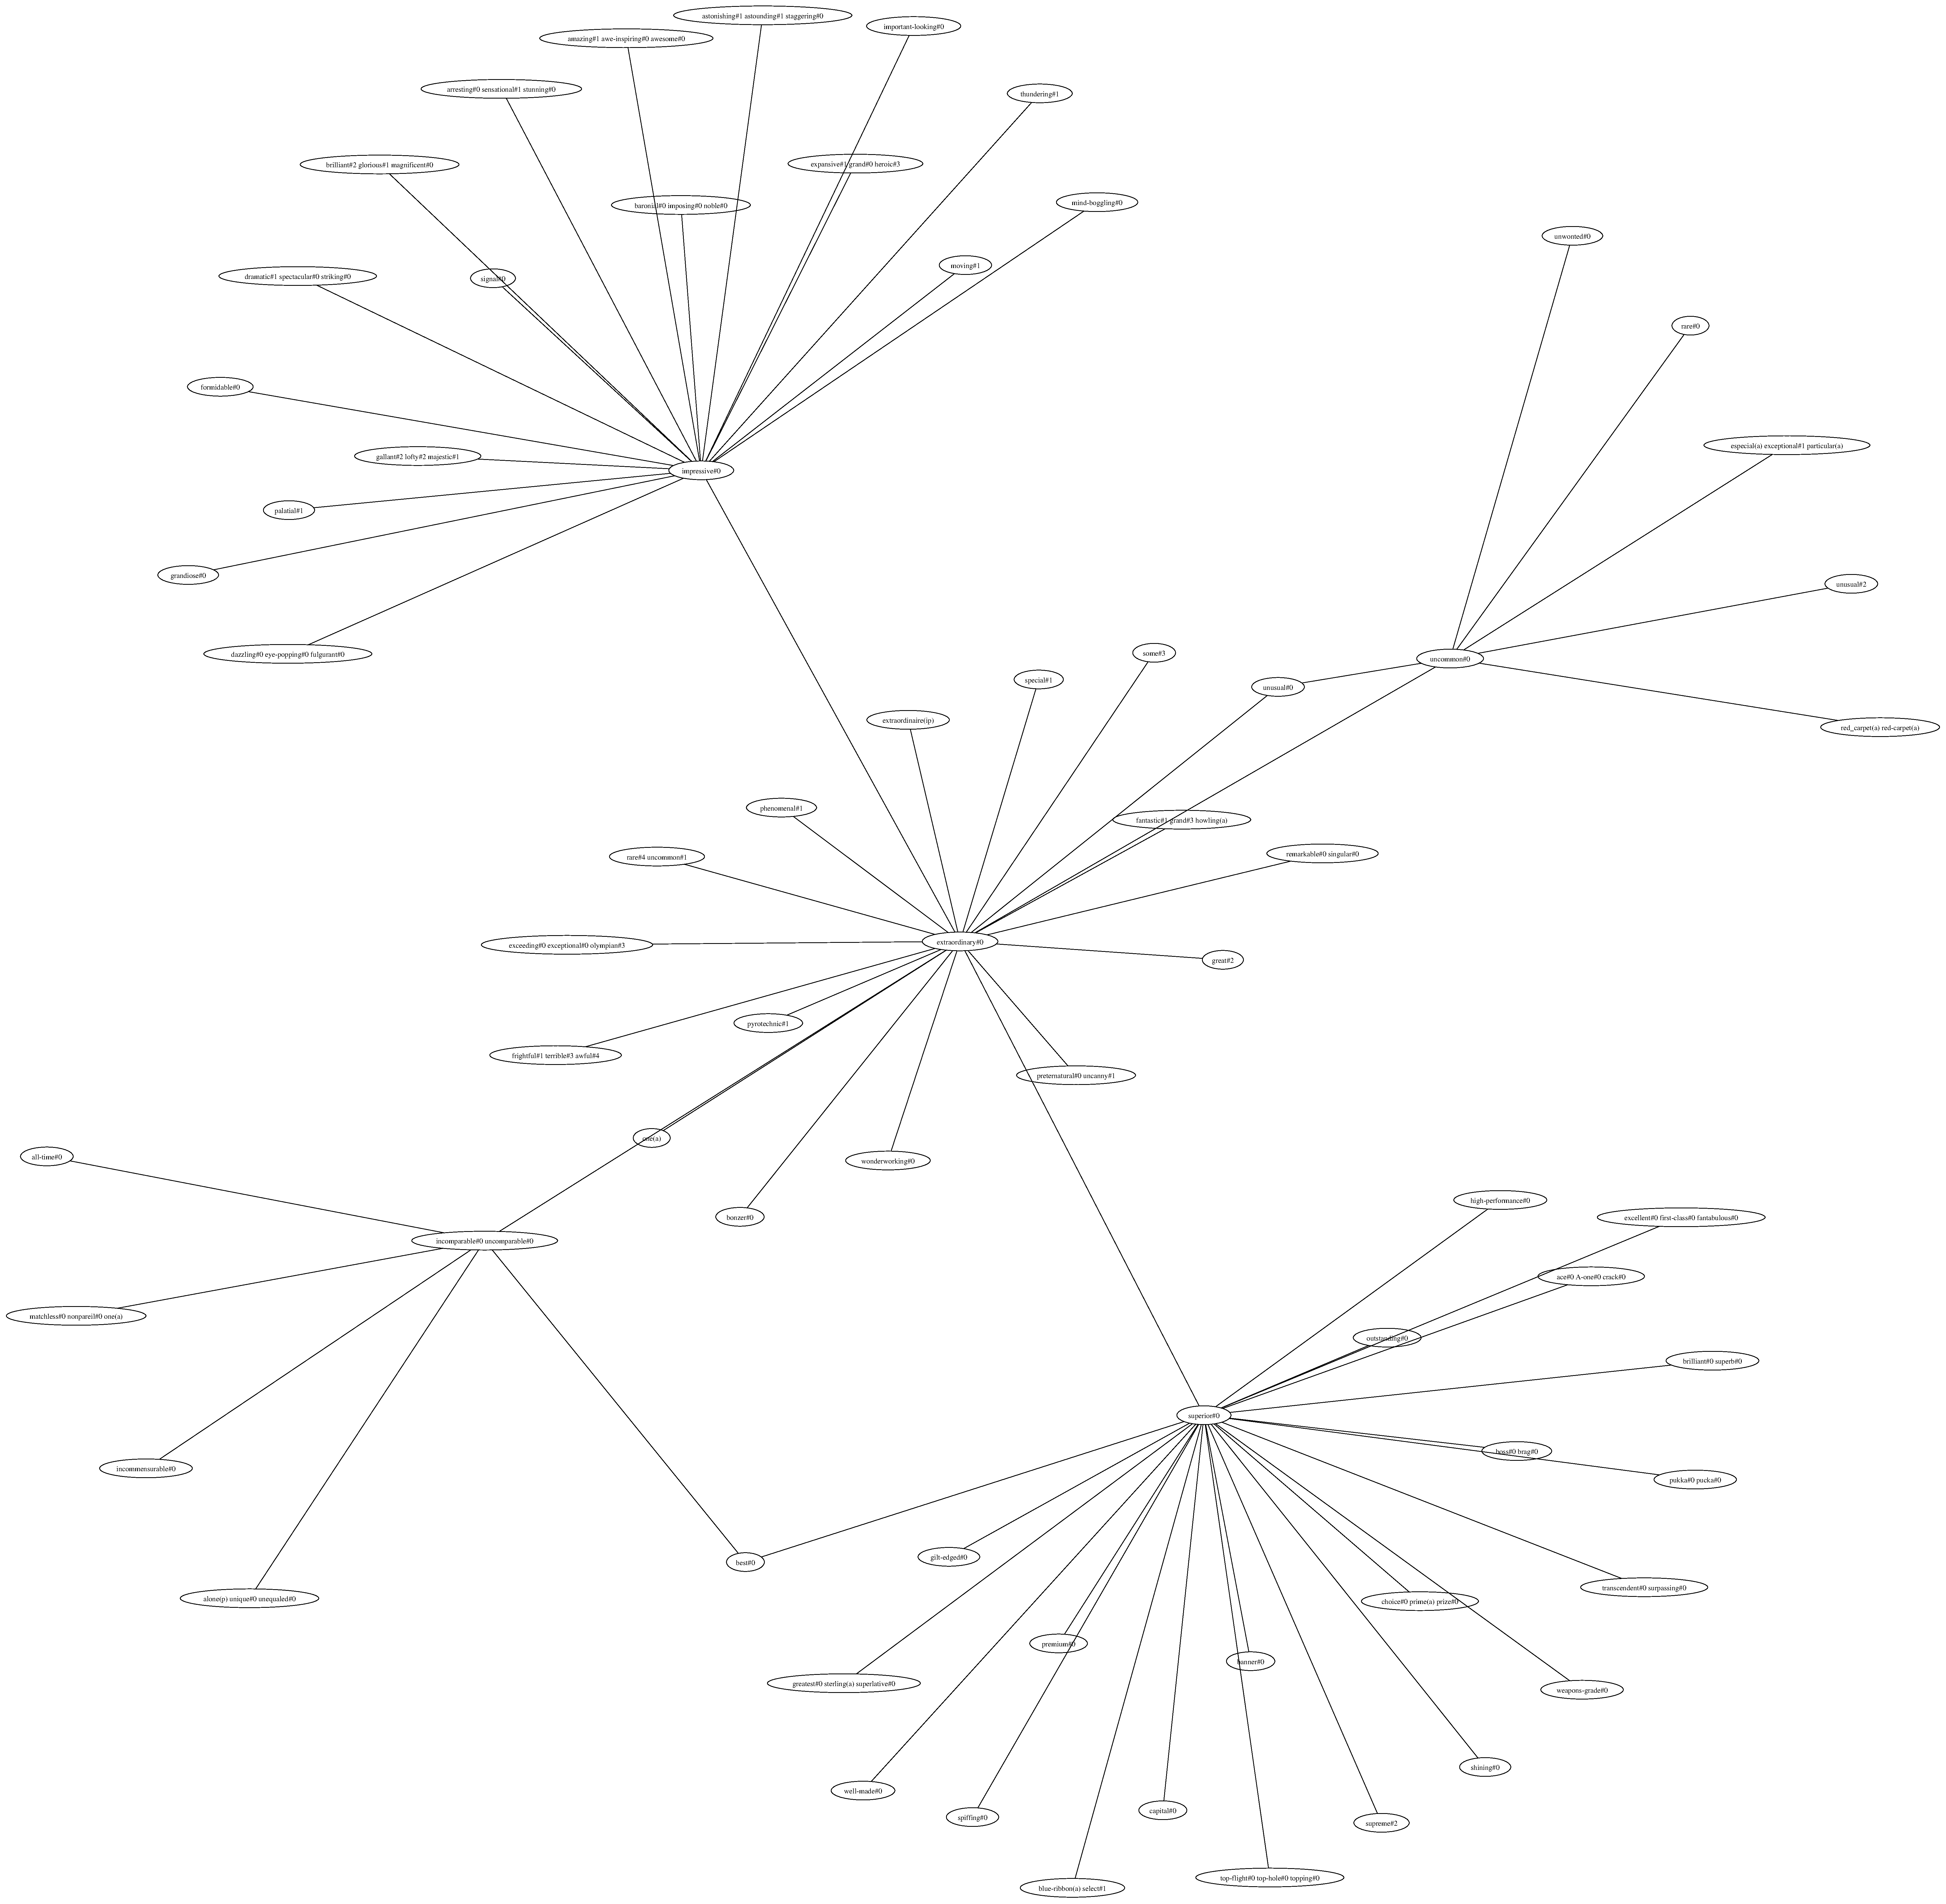
\includegraphics[scale=.4]{Figures/Exceptional}
\end{figure}

\cite[p. 453-456, 468, 471]{ai}

An illustrative example of such a graph, denoting a relation in a tiny semantic network of adjective concepts is given in figure X. The relation depictured . 
transitivity...


We have no way of detecting different semantic ambiguity, since we have no knowledge bade ... therefore we shall restrict our-self to 
%!TEX root = Thesis.tex

\lstdefinelanguage{GHC}{
	morekeywords={let,return,data,type,infix,deriving,class,where,do,instance},
	sensitive=true,
	morecomment=[l]{--},
	morestring=[b]",
}

\chapter{Implementation}
\label{chap:implementation}

In order to demonstrate the logical approach, introduced in the previous chapters, a \emph{proof of concept} system was implemented. In the following sections key aspects of the implementation of this system will be presented. A complete walk-though will not be presented, but the complete source code for the implementation is available in Appendix~\ref{code}. Also notice that code segments presented in this chapter maybe simplified from the source code to ease understanding. For instance the C\&C-toolchain uses some additional primitive categories to handle conjunctions, commas and punctuations that are not consider theoretical or implementationwise interesting, as they are translatable to the set of categories already presented. In the actual implementation of the proof of concept system this is exactly what is done, once the output from the C\&C-toolchain has been parsed.

It was chosen to use the purely functional programming language \emph{Haskell} for implementing the proof of concept system. The reason Haskell, specifically the \emph{Glasgow Haskell Compiler}, was chosen as programming language and platform, was i.a.\ its ability to elegantly and effectively implement a parser for the output of the C\&C-toolchain. Data structures are like in many other functional languages also possible to state in a very succinct and neat manner, which allow Haskell to model the extended semantics presented in Section~\ref{sec:extendingSemantics}, as well as any other structure presented, e.g.\ deduction proofs, lexical and phrasal categories, etc.

\section{Data structures}
Data structures are stated in Haskell by the means of \emph{type constructors} and \emph{data constructors}. To model for instance lexical and phrasal categories the two infix operators, \texttt{:/} and \texttt{:\textbackslash} are declared (using \texttt{/} and \texttt{\textbackslash} was not considered wise, as \texttt{/} is already used for devision by the Haskell Prelude) as shown in Figure~\ref{fig:categoryDataType}. The \emph{agreement} of an primitive category is simply a set of features cf. Section~\ref{sec:featuresAgreement}, which is easiest modeled using the list structure. As features are just values from some language specific finite set they are simply modeled by \emph{nullary data constructors}. One might argue that features have \emph{different} types, e.g.\ person, number, gender, etc. However it is convenient to simply regard all features as being of the \emph{same} type, a model borrow from \citeauthor{cs} \shortcite[chap.~9]{cs}. %Finally a category can by one of the four primitive categories, which are all \emph{unary data constructors} since they carry agreement, or a compound category using one of the infix operators.

\begin{figure}[ht]
\begin{cframed}{.9\textwidth}
\vspace{-8pt}
\begin{lstlisting}[language=GHC]
infix 9 :/  -- Forward slash operator
infix 9 :\  -- Backward slash operator

type Agreement = [Feature]

data Category = S Agreement             -- Sentence
              | N Agreement             -- Noun
              | NP Agreement            -- Noun Phrase
              | PP Agreement            -- Preposision Phrase
              | Category :/ Category    -- Forward slash
              | Category :\ Category    -- Backward slash

data Feature = SDcl | SAdj | SNb | SNg | ...
\end{lstlisting}	
\end{cframed}
\caption{Example of declaring the data structure for categories.}
\label{fig:categoryDataType}
\end{figure}

The code shown in Figure~\ref{fig:categoryDataType} is really all what is needed to represent the syntactic structure of categories. Another illustration of one of the data structural advantages of using a functional programming language is shown in Figure~\ref{fig:lambdaDataType}. Notice how the declaration of the syntax for the semantic expressions is completely analog to the formal syntax given in Definition~\ref{def:Lambda} and \ref{def:semanticExpressions}, with the exception that the implemented syntax is untyped. The reason why types are omitted from the implemented model of semantic expressions is simply that they are always accompanied by a category, and thus the type of the expression is trivially obtainable when needed.

\begin{figure}[ht]
\begin{cframed}{.9\textwidth}
\vspace{-8pt}
\begin{lstlisting}[language=GHC]
data SExpr = Var String                    -- Variable
           | Abs String SExpr              -- Lambda abstraction
           | App SExpr SExpr               -- Lambda application
           | Fun String Float Int [SExpr]  -- Functor
           | Seq [SExpr]                   -- Sequence
           | ImpactChange SExpr Int        -- Impact change
           | Change SExpr Float            -- Change
           | Scale SExpr Float             -- Scale
\end{lstlisting}	
\end{cframed}
\caption{Example of declaring the data structure for semantic expressions.}
\label{fig:lambdaDataType}
\end{figure}

\section{Reducing semantic expressions}

With data structures available for representing the syntax of the semantic expressions it is time to focus on reducing the expression using the semantic rules presented in Definition~\ref{def:semanticExpressions}. This can be easily done in a functional language by specifying a \emph{reduction function}, i.e.\ a function that recursively rewrites semantic expressions based on the rules presented in the definition. By using the \emph{pattern matching} available in Haskell, each rule can be implemented in a one-to-one manner by a function declaration that only accepts the \emph{pattern} of that rule. For instance Figure~\ref{fig:reduce} shows the implementation of the (FC1), (SC) and (PC) rules. A small set of additional function declarations are needed to allow reduction inside a structure that itself cannot be reduced, and finally the \emph{identity function} matches any pattern not captured by any of the other function declarations. Notice that $\eta$-reduction was not implemented, since this rule is merely a performance enhancing rule.
\begin{figure}[ht]
\begin{cframed}{.9\textwidth}
\vspace{-8pt}
\begin{lstlisting}[language=GHC]
-- (FC1)
reduce (Change (Fun f j 0 ts) j') = 
  Fun f (j + j') 0 $ map reduce ts

-- (SC)
reduce (Change (Seq ts) j') = 
  Seq $ map (reduce . flip Change j') ts

-- (PC)
reduce (Change (Abs x t) j') = 
  Abs x $ reduce $ Change t j'
\end{lstlisting}	
\end{cframed}
\caption{Example of declaring the rules for semantic expressions.}
\label{fig:reduce}
\end{figure}
\vspace{-1em}

\section{Parsing output from the C\&C tools}
The implemented parser for the Prolog style output yielded by the C\&C-toolchain, presented briefly in Section~\ref{sec:annotatingLexicon}, uses the \textsc{Parsec} library for Haskell by \citeauthor{parsec} \shortcite{parsec}. \textsc{Parsec} is a strong monadic parser combinator, that among other things allows fast and efficient parsing of LL[1] grammars, and can thus easily capture the subset of the Prolog language used by the C\&C-toolchain. \textsc{Parsec} differs significantly from common \textsc{Yacc} approaches, since it describes the grammar \emph{directly} in Haskell, without the need of some intermediate language or processing tools.

Figure~\ref{fig:candcOutputReal} shows the actual raw output from the C\&C-toolchain that is the basis the illustration in Figure~\ref{fig:candcOutput} shown back in Section~\ref{sec:annotatingLexicon}. The first section of the output represents the deduction tree, while the second represents the lexicon (obviously without semantic expressions).

\begin{figure}[ht]
\center
\begin{cframed}{.8\textwidth}
	\scriptsize
	\begin{verbatim}
ccg(1,
 ba('S[dcl]',
  fa('NP[nb]',
   lf(1,1,'NP[nb]/N'),
   lf(1,2,'N')),
  fa('S[dcl]\NP',
   lf(1,3,'(S[dcl]\NP)/(S[adj]\NP)'),
   lf(1,4,'S[adj]\NP')))).

w(1, 1, 'the', 'the', 'DT', 'I-NP', 'O', 'NP[nb]/N').
w(1, 2, 'service', 'service', 'NN', 'I-NP', 'O', 'N').
w(1, 3, 'was', 'be', 'VBD', 'I-VP', 'O', '(S[dcl]\NP)/(S[adj]\NP)').
w(1, 4, 'great', 'great', 'JJ', 'I-ADJP', 'O', 'S[adj]\NP').
	\end{verbatim}
\end{cframed}
\vspace{1em}
	\caption{Raw output from the C\&C toolchain.}
	\label{fig:candcOutputReal}
\end{figure}

One of the most admirable features of \textsc{Parsec} is its \emph{parser combinator library}, containing a verity bundled auxiliary functions, which allows the declaration of advanced parsers by combining smaller parsing functions. To parse for instance the categories present in both of the sections one can build an \emph{expression parser} simply by stating the \emph{symbol}, \emph{precedence} and \emph{associativity} of the operators.

Figure~\ref{fig:categoryExpression} shows the parser for categories. The precedence of the operators are given by the outer list in the \emph{operator table}, while operators within the same inner list have the same precedence, which is in the case for both of the categorial infix operators. Finally a category is declared as either compound (i.e.\ a category expression), or as one of the four primitive categories. Notice how the parser needs to first \emph{try} to parse \emph{noun phrases} (NP), and then \emph{nouns} (N), since the parser otherwise could successfully parse a noun, and then meet an unexpected ``P'', which would cause a parser error.

\begin{figure}[ht]
\begin{cframed}{.9\textwidth}
\begin{lstlisting}[language=GHC]
pCategoryExpr :: Parser Category
pCategoryExpr = buildExpressionParser pCategoryOpTable pCategory

pCategoryOpTable :: OperatorTable Char st Category
pCategoryOpTable = [ [ op "/"  (:/) AssocLeft, 
                       op "\\" (:\) AssocLeft ] ]
                   where 
                     op s f a = Infix ( string s >> return f ) a

pCategory :: Parser Category
pCategory =         pParens pCategoryExpr
            <|>     (pCategory' "S"     S)
            <|> try (pCategory' "NP"    NP)
            <|>     (pCategory' "N"     N)
            <|>     (pCategory' "PP"    PP)
            <?> "category" 
\end{lstlisting}	
\end{cframed}
\caption{Example of parsing categorial expression.}
\label{fig:categoryExpression}
\end{figure}
\vspace{1em}

The parsing of the lexicon is considered trivial, since its structure is flat with the exception of the category. ...

\todo[inline]{Finish}

\vspace{7em}

\section{WordNet interface and semantic networks}
To lookup semantic concepts and relations in the WordNet data files an open source interface library by \citeauthor{hwordnet} \shortcite{hwordnet} was used as base. However the interface was not complete, and missed critical features. For instance the library could only calculate the closure of two semantic concepts, which of cause only is possible when the relation forms a partial order, e.g.\ as is the case with the \emph{hyponym}/\emph{hypernym} relation and the \emph{holonym}/\emph{meronym} relation. Therefore the library has undergone significant rewrite and cleanup in order to use it for the presented purpose.

To model semantic networks another open source library was used, namely the \emph{Functional Graph Library} (FGL). The library implements efficient functional graph representation and algorithms presented by \citeauthor{fgl} \shortcite{fgl}. However transforming the relational representation of WordNet into an actual graph in the sense of FGL is somewhat tricky. The reason for this is that intended usage of the WordNet data files do not exposes $S$, and neither $r$ in the form of a subset of $S \times S$, which makes good sense since this representation does not scale well with $|S|$. Instead it is intended to query using the lookup function, $M$, which is indexed and allows logarithmic time lookup of lexical units; likewise a relation, $\hat{r}$, is a function from one semantic concept to a set of related concepts, i.e.\ $\hat{r}: S \to \mathcal{P}(S)$. This structure makes querying WordNet efficient, but also allows some optimization with respect to calculating the sentiment polarity value of lexical units. Recall from Section~\ref{sec:sentimentValue} that the approach is to select a set of respectively positive and negative seed concepts, and then measure the difference of the sum of distances from a lexical unit to these. However instead of regarding the entire graph $(S, r)$ only a subgraph $(S', r')$ is considered, namely the subgraph that constitutes the \emph{connected component} that contains all semantic concepts that are reachable from the seed concepts using the relation function $\hat{r}$. This of cause assumes that $r$ is symmetric, which is also the case for $r_\mathrm{similar}$ and $r_\mathrm{see\text{-}also}$ cf.\ Section~\ref{sec:sentimentValue}.

The construction of $(S', r')$ for some set of positive and negative semantic concepts, respectively $S_\mathrm{pos}$ and $S_\mathrm{neg}$, is denoted the \emph{unfolding} of $S_\mathrm{pos} \cup S_\mathrm{neg}$ using $\hat{r}$. It is done using simple depth first search with the set of initially ``unvisited'' semantical concepts $S_\mathrm{pos} \cup S_\mathrm{neg}$. The FGL requires nodes to be assigned a unique index, and also it is clearly neccessary to keep track of which semantical concepts has already been assigned a node in the graph, i.e.\ which nodes are considered visited. Lastely the set $S'$ and $r'$ should be incrementally build. In an imperative programming language maintaining such mutable state is straight forward, but in a purely functional programming language such as Haskell this require  . \citeauthor{st} \shortcite{st} presents a method to allow algorithms update internal state, while still externally be purely functional algorithms with absolutely no side-effects.

\begin{figure}[ht]
\begin{cframed}{\textwidth}
\begin{lstlisting}[language=GHC]
unfoldG :: (Ord a) => (a -> [a]) -> [a] -> (Map a Node, Gr a Int)
unfoldG r seeds = runST ( unfoldST r seeds )

unfoldST :: (Ord a) => (a -> [a]) -> [a] -> ST s (Map a Node, Gr a Int)
unfoldST r seeds =
    do mapRef    <- newSTRef Map.empty    -- Map from Item to Node
       nodesRef  <- newSTRef []           -- List of Node/[Edge] pairs
       idRef     <- newSTRef 0            -- Counter for indexing nodes
       -- Recursively visits n
       let visit n = 
             do -- Test if n has already been visited
                test <- (return . Map.lookup n =<< readSTRef mapRef)
                case test of
                  Just v  -> return v
                  Nothing -> do -- Get next id for this item
                                i <- readSTRef idRef
                                modifySTRef idRef (+1)
                                -- Update item/node map
                                modifySTRef mapRef (Map.insert n i)
                                -- Recursively visit related items
                                ks <- mapM visit $ r n 
                                let ns = ((i,n), [(i,k,1) | k <- ks])
                                modifySTRef nodesRef (ns:)
                                return i
       -- Visit seeds
       mapM visit seeds
       -- Read resuls and return map/graph-pair
       list <- readSTRef nodesRef         
       nodeMap <- readSTRef mapRef
       let nodes = [n | (n, _) <- list]
       let edges = concat [es | (_, es) <- list]
       return (nodeMap, mkGraph nodes edges)
\end{lstlisting}  
\end{cframed}
\caption{Example of parsing categorial expression.}
\label{fig:categoryExpression}
\end{figure}

\todo[inline]{Finish}

%... the function for calculating the closure of synsets $S$ for some relatrion $R$ does not terminate if $R$ is symmetric. Since several semantic relations are symmetric (e.g. synonyms, antonyms)


Note: Appendix med kildekode -- komplet oversigt over filer / ansvar -- Udvalgte filer inkluderet.

%!TEX root = Thesis.tex

\chapter{Test results}
\label{chap:testResults}

%!TEX root = Thesis.tex

\chapter{Discussion}
\label{chap:Conclusion}

Even though the stucture of the sentences is inspected deeply though the syntactic analysis the semantic expression assigned to adjectives and adverbs is still atomic, and based on the key concepts the the context specific positive and negative lists. Even though the lists are context specific, a concept can have ... løses dette evt. af subject-focus?


Since adjectives and adverbs are always reduced to only contribute to the polarity, they cannot be used to identify subjects. E.g. what do you think about the white iPhone vs. the black? (need bette ex.!)

\section{Fureture work}
We expect such an algorithm to calculate a match score, that is a weighted average over several metrics. Given below are methods for calculating scores for some evident metrics.

\begin{itemize}
  \item Symbolic similarity -- at its most basic form we can consider a sample string (i.e. a word from an input text) against the system's vocabulary using approximate string matching algorithms such as the  \emph{Levenshtein distance} as described by \cite{Wagner}.

  \item Pronunciation similarity -- it is an valid assumption that many misspellings still share a majority of the pronunciation with the intended word, i.e. they are approximately homophone. Thus comparing the phonetic properties of an sample string with possible matches can in cases correct misspellings. The \emph{Soundex algorithm} by Robert C. Russell and Margaret K. Odell, as described by \cite[p. 391–92]{ACP3}, is a simple, yet power full approach for this purpose.

\end{itemize}

---

``lift'' restrictions about the texts, e.g. no of sentences ... context-sensitive, e.g. resolution of relative pronpoun ... The room was luxurious, it had ...

\chapter{Conclusion}
\label{chap:Conclusion}
\appendix
%!TEX root = Thesis.tex
\chapter{A naive attempt for lexicon acquisition}
\label{chap:brownCorpus}

This appendix describes the efforts that was initially made in order to acquire a CCG lexicon by \emph{transforming} a tagged corpus, namely the \emph{Brown Corpus}. The approach turned out to be very naive, and was dropped in favor for the C\&C models trained on the CCGBank \cite{ccgBank}, in turn The Penn Treebank \cite{pennTreebank}.

\section*{The Brown Corpus}
English is governed by convention rather than formal code, i.e.\ there is no regulating body like the Académie française. Instead, authoritative dictionaries, i.a.\  Oxford English Dictionary, describe usage rather than defining it. Thus in order to acquire a covering lexicon it is necessary to build it from large amount English text.

The Brown Corpus was compiled by \citeauthor{brown} \shortcite{brown} by collecting written works printed in United States during the year 1961. The corpus consists of just over one million words taken from 500 American English sample texts, with the intension of covering a highly representative variety of writing styles and sentence structures.

Notable drawbacks of the Brown Corpus include its age, i.e.\ there are evidently review topics where essential and recurring words used in present day writing was not coined yet or rarely used back 50 years ago. For instance does the Brown Corpus not recognize the words \emph{internet}. However it is one of the only larger \emph{free to use} tagged corpus available, and for this reason is was chosen for the attempt. Even early analysis showed that coverage would be disappointing, since the Brown Copus only contains 80.4\% of the words of the \emph{hotels and restaurants} subset of the \emph{Opinosis data set} \cite{Opinosis} ($\num{3793}$ words). This mean that every 5th word would on average be a guess in the blind. However the approach was continued to see how many sentences would be possible to syntactic analyze with the lexicon.

The corpus is annotated with \emph{part of speech} tags, but does not include the deep structure of a \emph{treebank}. There is a total of 82 different tags, some examples are shown in Table~\ref{tab:brownTags}. As shown from the extract the tags include very limited information, and while some features can be extracted (e.g.\ tense, person) in some cases, the tagging gives no indication of the context.
\begin{table}[ht]
\begin{center}
\begin{tabular}{ll}
  Tag & Description \\ \hline \hline
  VB  & verb, base form \\ \hline
  VBD & verb, past tense \\ \hline
  VBG & verb, present participle/gerund \\ \hline
  VBN & verb, past participle \\ \hline
  VBP & verb, non 3rd person, singular, present \\ \hline
  VBZ & verb, 3rd. singular present 
\end{tabular}
\end{center}
\caption{Extract from the Brown tagging set.}
\label{tab:brownTags}
\end{table}

Without any contextual information the approach for translating this information into lexical categories is becomes very coarse. For instance there are no way of determining whether a verb is \emph{intransitive}, \emph{transitive}, or \emph{di-transitive}. The chosen method was simply to over-generate, i.e. for every verb entries for all three types of verbs was added to the lexicon. In total 62 of such rules were defined, which produced a lexicon containing CCG categories for 84.5\% of $\num{56057}$ unique tokens present in the Brown Corpus.

\section*{Evaluating the lexicon}
To evaluate the coverage of the acquired lexicon an \emph{shift-reduce} parser was implemented in Haskell. It is not the most effective parsing strategy, but was simple to implement and considered efficiently enough to test the lexicon. A representative sample of the \emph{hotels and restaurants} subset of the \emph{Opinosis data set} was selected (156 sentences). The result was that the parser only was able to parse $10.9\%$ of the sentences. The result was very disappointing, and it was not even considered weather these even was correctly parses. Insted it was recognized that building a CCG lexicon from only a tagged corpus is not a feasible approach. Further development of the approach was dropped and instead the component was replaced with the C\&C~tools~\cite{candc}.



							              %Appendix A
%%!TEX root = Thesis.tex
\newcommand{\source}{../Code/CC}
\chapter{Source code}
\label{chap:source}

Complete source code for the proof of concept solution presented can be downloaded from the url: \url{http://www.student.dtu.dk/~s072466/msc.zip}.

The following lists the essential Haskell code files for the implementation. \texttt{Main.hs} defines the extraction and analysis algorithms, i.e. $\mathcal{E}$ and $\mathcal{A}$, and also includes the main entry point for the application. The syntax and semantics for the semantic expressions are defined in \texttt{Lambda.hs}. The implementation of Combinatory Categorial Grammar (CCG) is defined by \texttt{CCG.hs}, and \texttt{Annotate.hs} defines both the generic annotation algorithm $\mathcal{U}_\textsc{gen}$, as well as the special case annotation algorithms. Finally \texttt{Parser.hs} defines the parser for the output from the C\&C toolchain. The following listing thus thereby not include the WordNet interface.

\section*{Main.hs}
\lstinputlisting[basicstyle=\tiny]{\source/Main.hs}

\section*{Lambda.hs}
\lstinputlisting[basicstyle=\tiny,inputencoding=utf8/latin1]{\source/Lambda.hs}

\section*{CCG.hs}
\lstinputlisting[basicstyle=\tiny,inputencoding=utf8/latin1]{\source/CCG.hs}

\section*{Annotate.hs}
\lstinputlisting[basicstyle=\tiny,inputencoding=utf8/latin1]{\source/Annotate.hs}

\section*{Parser.hs}
\lstinputlisting[basicstyle=\tiny,inputencoding=utf8/latin1]{\source/Parser.hs}

                           %Appendix B
%!TEX root = Thesis.tex
\chapter{Labeled test data}
\label{chap:testData}

The following table consists of a random sample chosen from the ``Swissotel Hotel'' topic of the \emph{Opinosis data set} \cite{Opinosis} which contain any morphological form of the \emph{subject of interest: hotel rooms}. Each sentence in the data set (which may not constitute a complete review) has been labeled independently by two human individuals \emph{with respect to the subject of interest: hotel rooms}. Furthermore the table contains results for the baseline (sentence level polarity value), and results for the presented method (entity level polarity value of subject of interest).

%\begin{table}[f]
\begin{landscape}
\begin{center}
\small % scriptsize
\begin{longtable}{rm{9cm}ccc}
\# & Review text & Human A & Human B & Presented method \\
\hline\hline
\endhead
1 & The rooms are in pretty shabby condition , but they are clean . 
& Negative & Negative & Unknown \\ \hline
2 & The rooms are spacious and have nice views, I was NOT impressed with the mattress and every, little, tiny thing costs money . 
& Unknown & Unknown & N/A \\ \hline
3 & The rooms look like they were just remodled and upgraded, there was an HD TV and a nice iHome docking station to put my iPod so I could set the alarm to wake up with my music instead of the radio .
& Positive & Positive & Unknown \\ \hline
4 & The rooms were cleaned spic and span every day .
& Positive & Positive & Unknown \\ \hline
5 & When I got to the room , I thought the new rooms would have a plasma since the website implies the new rooms would have them , but I guess those come later .
& Negative & Negative & Unknown \\ \hline
6 & Very impressed with rooms and view !
& Positive & Positive & Unknown \\ \hline
7 & The rooms are not all that big .
& Negative & Negative & Unknown \\ \hline
8 & Expensive Parking but great rooms .
& Positive & Positive & $10.0$ \\ \hline
9 & Rooms were nicely furnished .
& Positive & Positive & Unknown \\ \hline
10 & The rooms are very clean , comfortable and spacious and up-to-date .
& Positive & Positive & $65.0$ \\ \hline
11 & I've olny ever stayed in the ``standard'' rooms in this property , all of which are spacious and airy , and function well for both business or leisure travellers .
& Positive & Positive & Unknown \\ \hline
12 & It does suffer , however , from a trend that I have been noticing that as rooms at business class hotels are upgraded ,  particularly with a patch panel for the big LCD , TV , drawer space becomes less and less .
& Negative & Negative & Unknown \\ \hline
13 & We even got upgraded to one of the corner rooms which also looked west toward Michigan Ave and the Wrigley building .
& Positive & Positive & Unknown \\ \hline
14 & The rooms were very clean , the service was polite and helpful , and it's near the heart of Chicago !
& Positive & Positive & $45.0$ \\ \hline
% Page 2
15 & You can see downtown and or the Navy Pier from most of the rooms .
& Positive & Positive  & Unknown \\ \hline
16 & no more bathrobes in corner rooms suites , coffee service in room is parred way down , the buffet offered in the cafe is not as bountiful , although the cafe staff is inpeccable and extremely gracious and will bring you what you wish , check in staff not at all eager to upgrade you, even though you may be a frequent visitor .
& Negative & Negative  & Unknown \\ \hline
17 & Our rooms were nice and didn't look worn or old .
& Positive & Positive  & Unknown \\ \hline
18 & Rooms at the hotel are getting somewhat tired .
& Negative & Negative & TODO! (Positive)\\ \hline
19 & Great Location great rooms and bed but no help from desk personnel .
& Positive & Positive & $30.0$ \\ \hline
20 & While the rooms are quite nice , I was dismayed by the snotty service I received at the Swissotel in Chicago .
& Positive & Positive & $70.0$ \\ \hline
21 & Rooms are dated , our corner room's bathroom was shabby .
& Negative & Negative & Unknown \\ \hline
22 & The hotel was very nice , rooms were big , the pool hot tub area was very nice , and the location was great and easy to get to .
& Positive & Positive & Unknown \\ \hline
23 &Rooms are good quality and clean , what you would expect from a four star business hotel .
& Positive & Positive & $45.0$ \\ \hline
24 &The view from the rooms was fantastic , My daughters are allergic to feathers and all trace of them were removed from the room as soon as we advised housekeeping .
& Positive & Positive & Unknown \\ \hline
25 & The Swissotel is one of our favorite hotels in Chicago and the corner rooms have the most fantastic views in the city .
& Positive & Positive & Unknown \\ \hline
26 & Then again , the rooms are much larger and the view more than makes up for it .
& Positive & Positive & $65.0$ \\ \hline
27 & Rooms in similar hotels would usually be about \$250 , 300 .
& Positive & Positive & Unknown \\ \hline
28 & The actual hotel and rooms were very nice with amazing views , the staff was extremely rude .
& Positive & Positive & Unknown \\ \hline
29 & The rooms were clean , and upscale for the low price we paid .
& Positive & Positive & Unknown \\ \hline
% Page 3
30 & Thanks to TravelZoo I was able to find an amazing deal , lakeside rooms for \$129 night as part of a spring promotion .
& Positive & Positive & Unknown \\ \hline
31 & I recieved a great deal on the rooms here and it was wonderful .
& Positive & Positive & $20.0$ \\ \hline
32 & The room was huge as hotel rooms go .
& Positive & Positive & $65.0$ \\ \hline
33 &Hotel was very clean and the rooms were comfy .
& Positive & Positive & Unknown \\ \hline
34 & word to the wise , avoid the rooms ending with 11 .
& Negative & Negative & Unknown \\ \hline
35 & The rooms are large and well , appointed , the staff was very professional and friendly , and the view was striking ! 
& Positive & Positive & $40.0$\\
\caption{Labeled test data, subject of interest: Room}
\label{table:labeling}
\end{longtable}
\end{center}
\end{landscape}

%\end{sidewaystable}
                             %Appendix B
%-----------
% Backmatter
%-----------d
\backmatter
\chaptermark{Bibliography}
\renewcommand{\sectionmark}[1]{\markright{#1}}
\sectionmark{Bibliography}
\addcontentsline{toc}{chapter}{Bibliography}        %Force addition of Bibliography to TOC
\bibliographystyle{named}                           %Use alpha codes for references
\bibliography{References}    	                      %Bibliography file called
\end{document}
% % % EOF % % %